\chapter{Encabiments isomètrics del tor pla}
\section{Introducció al capítol}
Al capítol anterior hem enunciat i demostrat els teoremes d'encabiments isomètrics $C^1$ de Nash, i hem vist la manera en què Kuiper va reduir la codimensió de l'espai ambient a 1. A continuació revisitarem el tor, una varietat topològica que no es pot encabir isomètricament de manera suau en $\mathbb R^3$, com hem vist al capítol \ref{cap:intro}, i descriurem el mètode amb el qual es pot encabir isomètricament de manera $C^1$. 
Veurem que aquesta demostració ja utilitza el llenguatge de la integració convexa, que hem introduït al final del capítol anterior.

L'elaboració d'aquest encabiment va ser realitzada per Vincent Borrelli, Saïd Jabrane, Francis Lazarus i Boris Thibert i publicada l'any 2013. La cita principal d'aquest capítol és \cite{borrelli2013}. En aquest capítol no donem, en general, les demostracions de lemes i sublemes, que es troben a \cite{borrelli2013}.

\section{Integració convexa 1D}
A continuació exposarem el mètode d'integració convexa en el cas 1D, que és el cas més senzill i servirà de base per a la integració convexa en el cas 2D. Veurem que consisteix en trobar solucions de relacions diferencials a partir de termes oscil·lants d'alta freqüència, que anomenarem voltes. A més, donarem la funció exacta que determina aquestes voltes, en el cas dels encabiments isomètrics.

\begin{defi}
    Per cada $x\in I := [0,1]$, sigui $\mathcal R_x$ un conjunt de vectors en $\mathbb R^n$. Anomenem \textbf{relació diferencial} a la unió $\mathcal R := \bigcup_{x\in I} \mathcal R_x$. Anomenem \textbf{solució de} $\mathcal R$ a una corba $f:I\to\mathbb R^n$ de classe $C^1$ tal que $f'(x)\in\mathcal R_x$ per a tot $x\in I$.
\end{defi}

El mètode d'Integració Convexa ens permetrà trobar solucions de relacions diferencials arbitràriament properes a corbes $f:I\to\mathbb R^n$ de classe $C^1$ qualssevol. Per a això necessitarem una família de funcions que aproximin el comportament de la derivada de la següent manera:

\begin{defi}
    Sigui $f:I\to\mathbb R^n$ una corba de classe $C^1$. Anomenem \textbf{volta} de $f$ a una funció $h(x, \cdot): \mathbb R / \mathbb Z \to \mathcal R_x$ tal que
    \begin{equation}\label{eq:def voltes}
        f'(x) = \int_0^1 h(x, u)  du,
    \end{equation}
    és a dir, tal que la derivada $f'(x)$ és la mitjana de la volta $h(x, \cdot)$ sobre el cercle unitat.
\end{defi}

Si aquestes voltes existeixen, podem utilitzar-les per obtenir una nova aplicació que aproxima $f(t)$.
\begin{defi}
    Sigui $f:I\to\mathbb R^n$ una corba de classe $C^1$ i $h(x, \cdot)$ una volta de $f$. Anomenem \textbf{integral convexa} de $h$ a la funció $F:I\to\mathbb R^n$ donada per
    \begin{equation*}
        F(t) := f(0) + \int_0^t h(x, \set{Nx})  dx,
    \end{equation*}
    on $\set{Nx}$ és la part fraccionària de $Nx$.
\end{defi}    

\begin{figure}[htbp]
    \centering
    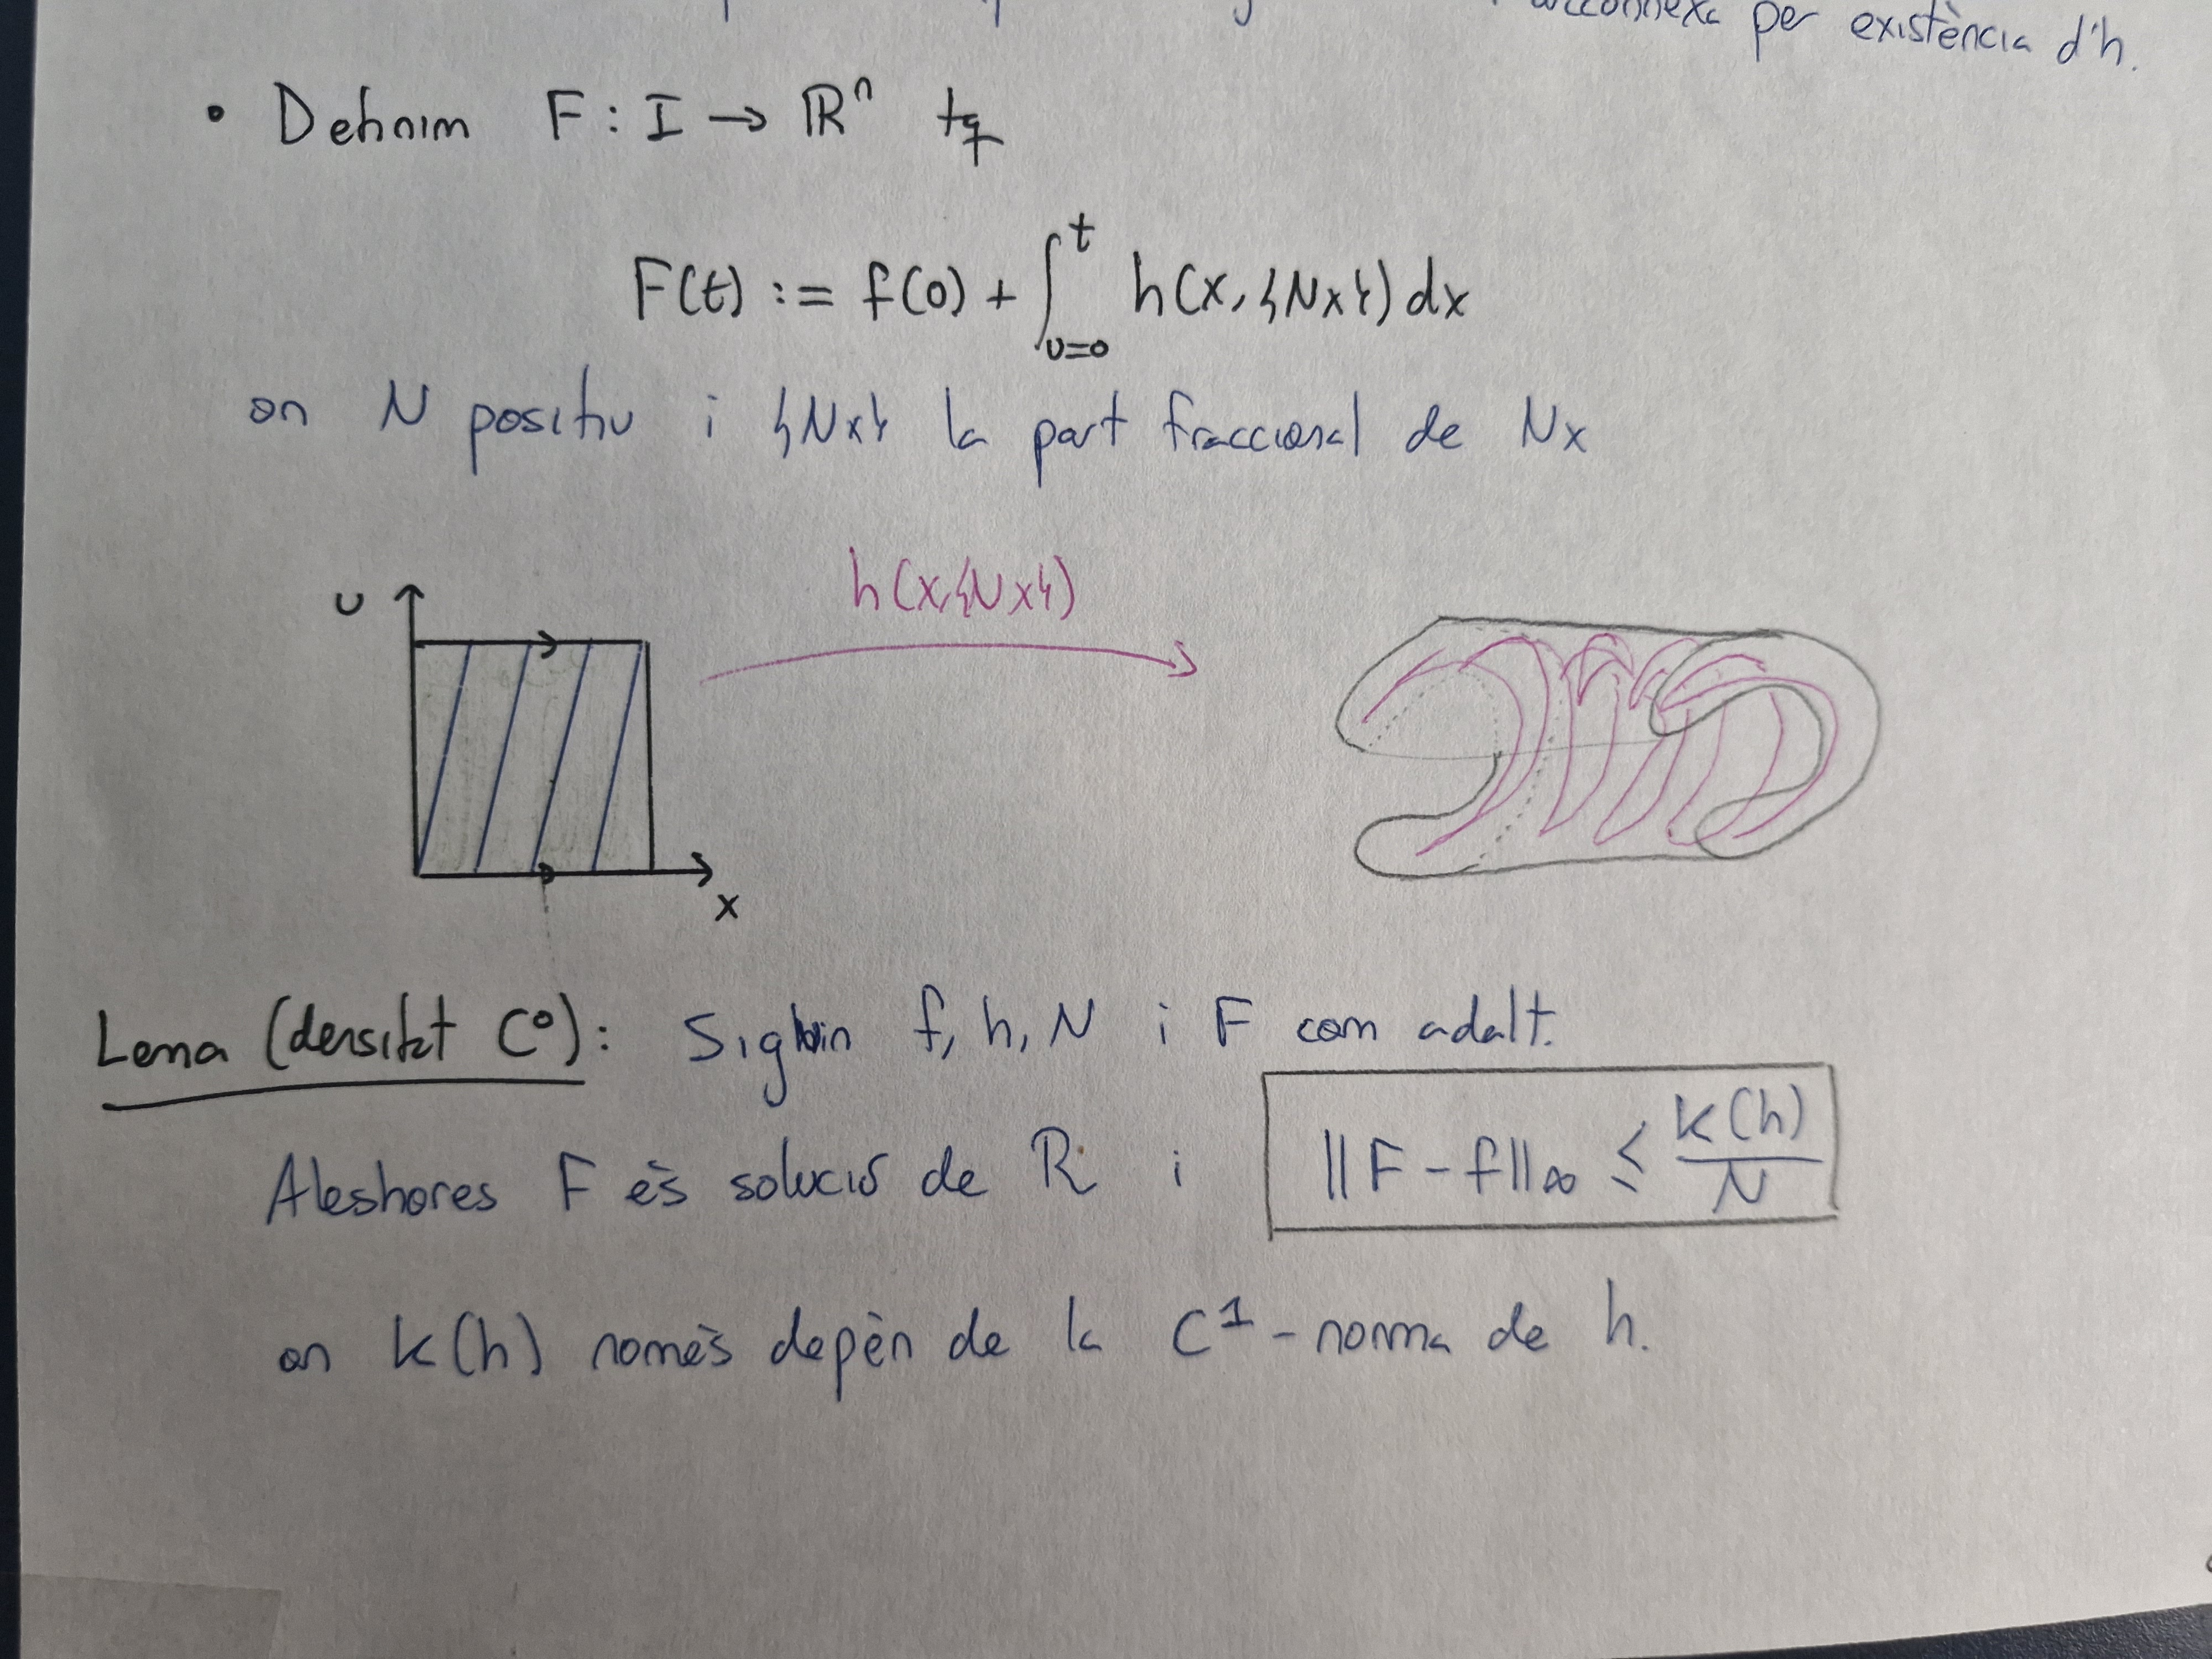
\includegraphics[width=0.5\textwidth]{Fotos/CINQUENA.jpg}
    \caption{{\color{blue}TEXT}}
    \label{fig:cinquena_foto}
\end{figure}

Intuïtivament, $F$ s'obté integrant $h$ sobre una corba de període $1/N$, de tal manera que per $N$ molt gran, cada període és proper a una volta concreta $h(x, \cdot)$, i per tant la seva integral és propera a $f'(x)$. D'aquesta manera, l'efecte acumulat per totes les voltes és proper a $f(t)$, i s'aproxima a $f(t)$ per $N$ molt gran. 
\begin{obs}
    El rol d'aquesta variable $N$ és similar al rol de la variable $\lambda$ en els mètodes de Nash i de Kuiper: a mesura que creix $N$, $F$ oscil·la més ràpidament i aproxima millor $f(t)$.
\end{obs}

\begin{lema}\label{lema:C0-1D}
    Siguin $f$, $h$, $N$ i $F$ com hem definit més amunt. Aleshores, $F$ és solució de la relació diferencial $\mathcal R$ i 
    \begin{equation}
    \|F-f\|_{C^0} \le \frac{K(h)}{N},
    \end{equation}
    on $K(h)$ només depèn de $\|h\|_{C^1}$.
\end{lema}

Tal com hem definit les relacions diferencials més amunt, veiem que restringeixen els valors que pot prendre la derivada $f'$ al llarg de la corba. En el nostre cas, ens interessa mantenir la derivada prou petita, per tal que en cada etapa d'integració convexa la nostra aplicació segueixi sent curta. Així, les nostres relacions diferencials $\mathcal R_s$ seran esferes de radi $r(s)>0$ en $\mathbb R^n$ prou petites. En concret, tindrem corbes $f$ que seran curtes si i només si $\|f'(s)\|\le r(s)$.

Suposant que $f'$ mai s'anul·la, podem definir $\vec n:I\to\mathbb R^n$ un vector normal a $f'$ i $\vec t(s):=f'(s)/\|f'(s)\|$. Podem fer ús d'aquests vectors per definir les voltes $h(s, \cdot)$ de la següent manera:
\begin{equation*}
    h(s, u) = r(s)(\cos(\alpha_s\cos(2\pi u))\vec t(s) + \sin(\alpha_s\sin(2\pi u))\vec n(s)),
\end{equation*}
on $\alpha_s := J_0^{-1}(\|f'(s)\|/r(s))$, on $J_0$ és la funció de Bessel de primer tipus i d'ordre 0. Per la propietat
\begin{equation*}
    J_0(x) = \int_0^1 \cos(x\cos(2\pi u)) du,
\end{equation*}
es verifica la condició de l'equació \eqref{eq:def voltes}.

\begin{figure}[htbp]
    \centering
    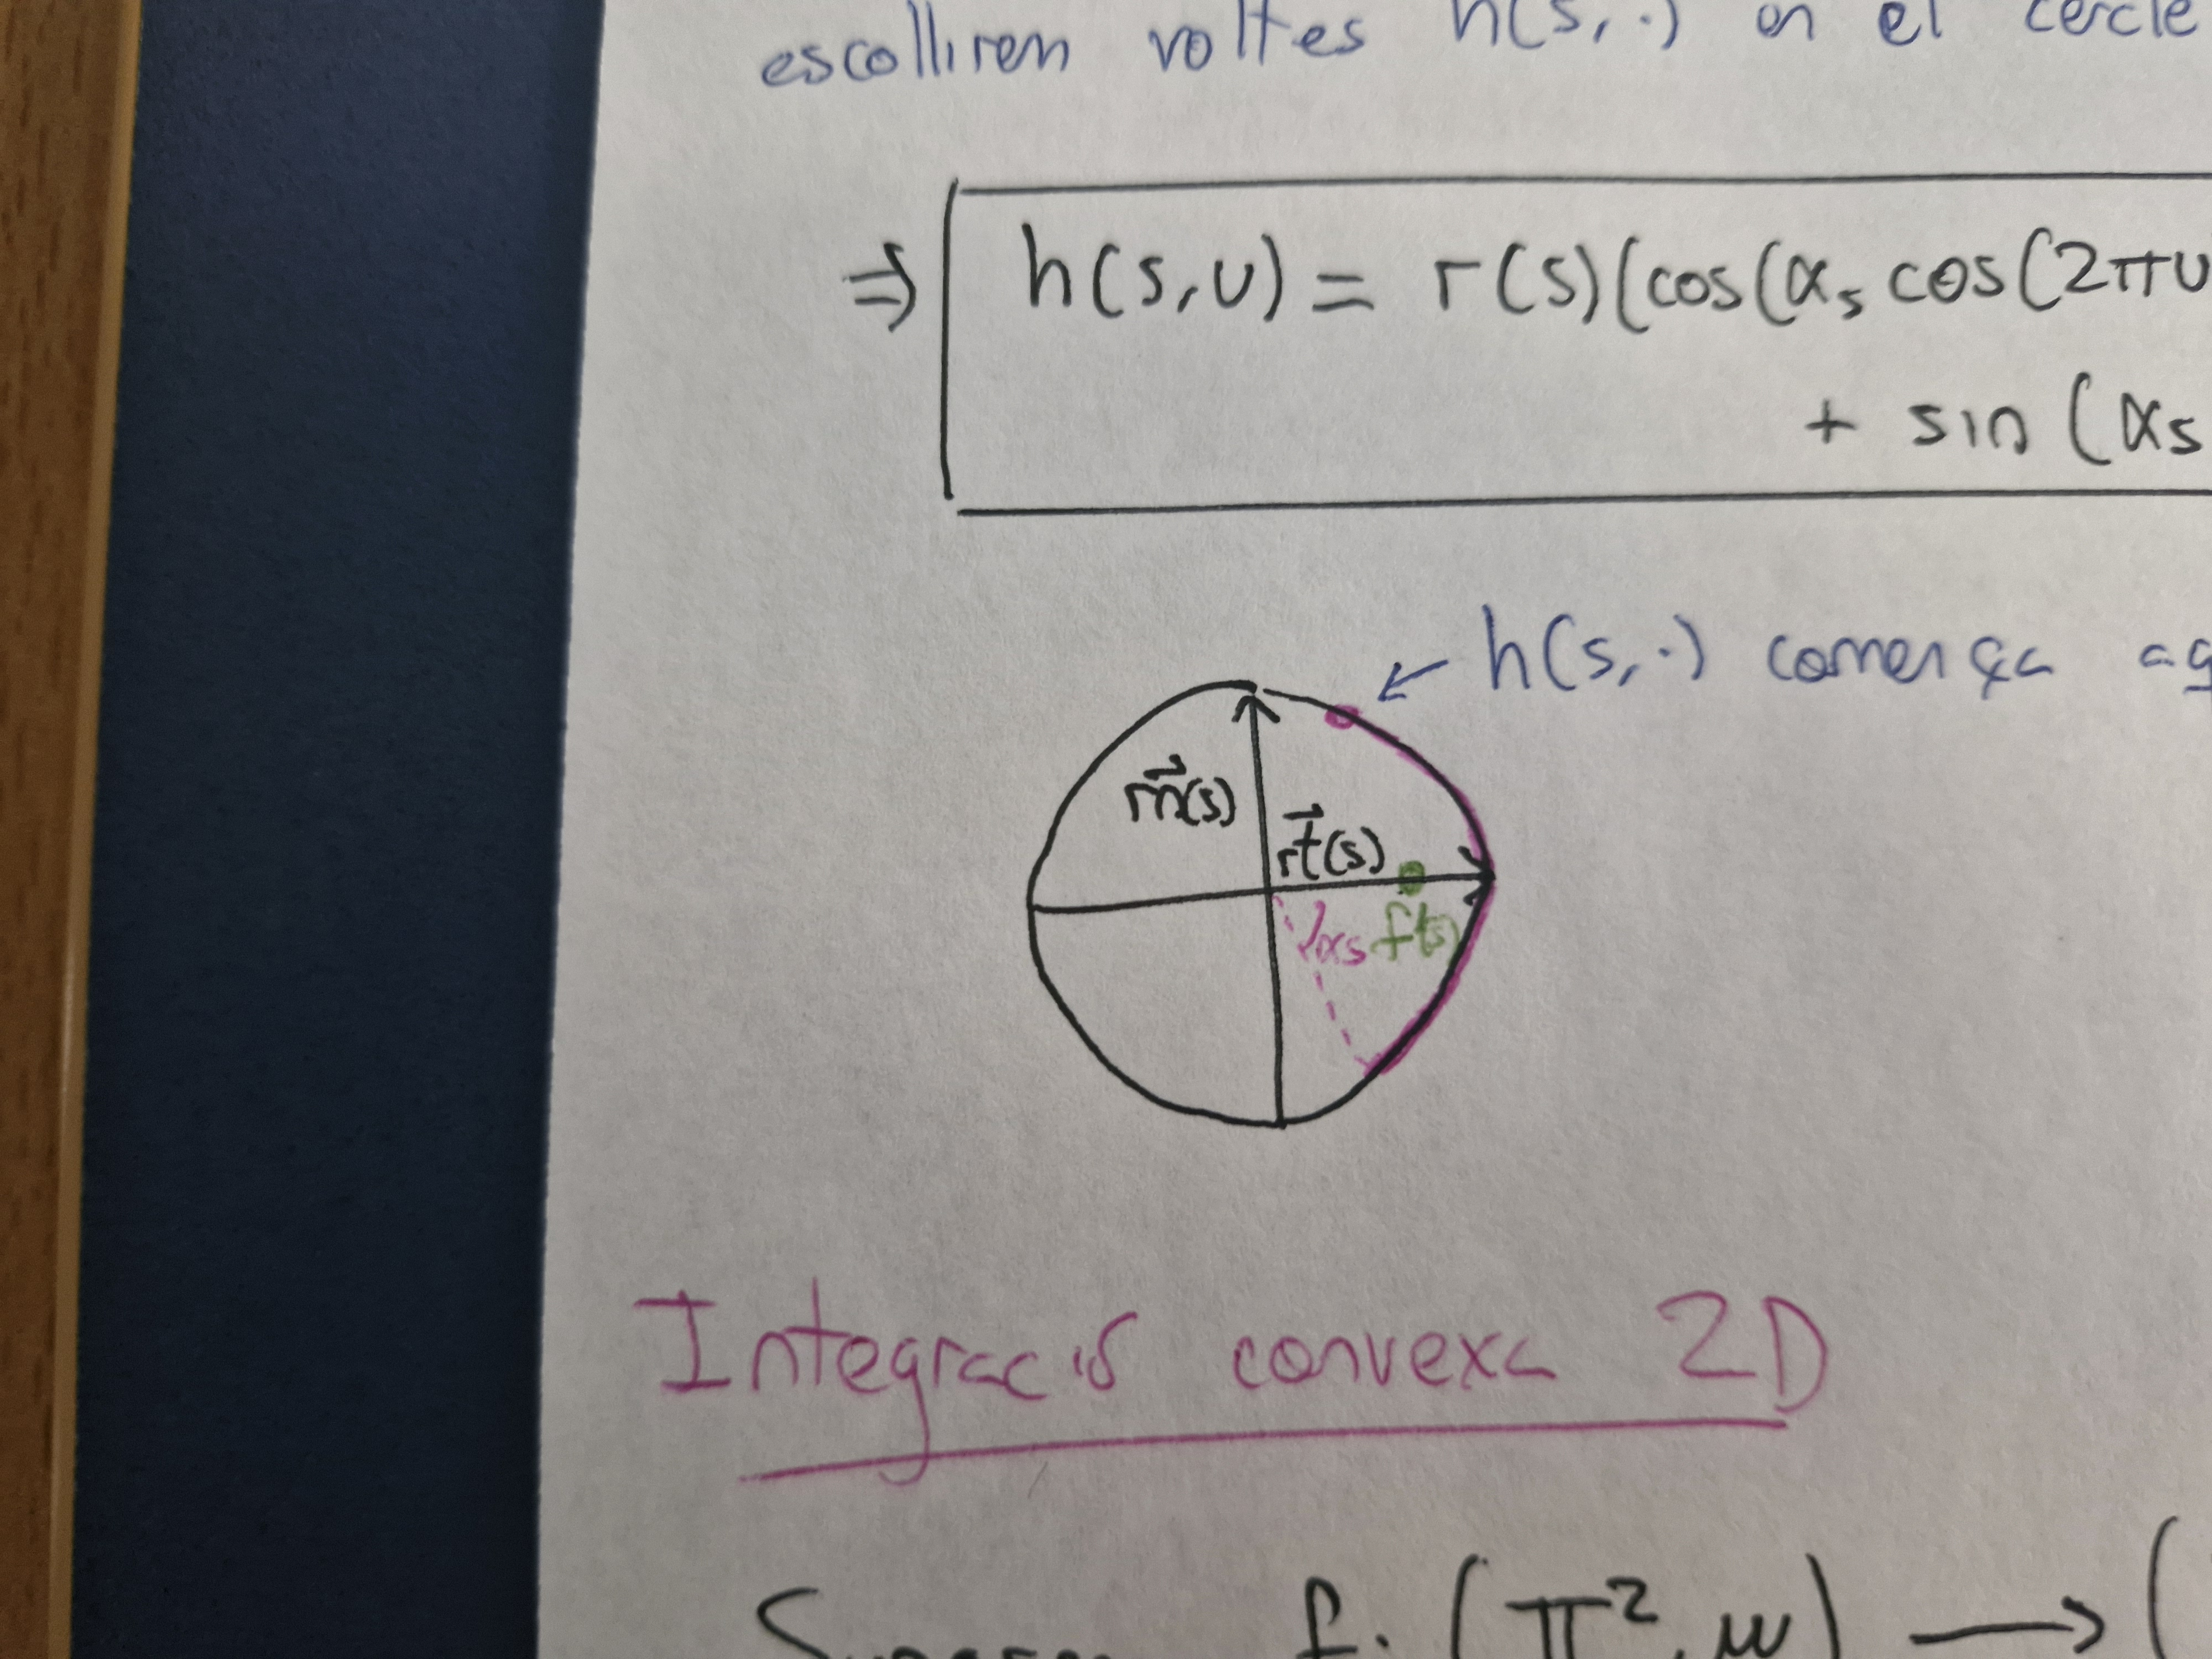
\includegraphics[width=0.5\textwidth]{Fotos/SISENA.jpg}
    \caption{{\color{blue}TEXT}}
    \label{fig:sisena_foto}
\end{figure}

\section{Integració convexa 2D: el cas primitiu}
Havent vist com es troba un encabiment isomètric mitjançant Integració Convexa en el cas 1D, ara veurem com es pot fer en el cas 2D. Intuïtivament, considerarem la superfície resultant d'un encabiment com una família de corbes unidimensionals, per tal de poder aplicar el resultat del lema \ref{lema:C0-1D} a cada una d'elles.

Considerem el problema que volem resoldre, és a dir, trobar un encabiment isomètric d'un tor $\mathbb T^2 = \mathbb R^2/\mathbb Z^2$ amb una mètrica $\mu$ en l'espai euclidià tridimensional. Com hem fet en la demostració del teorema de Nash al capítol anterior, partirem d'un encabiment inicial curt $f:(\mathbb T^2, \mu)\to(\mathbb R^3, \langle\cdot, \cdot\rangle)$ de classe $C^\infty$. Abans de considerar el cas més general, però, partirem primer de la suposició que la diferència entre la mètrica $\mu$ i el \textit{pullback} de la mètrica euclidiana per $f$ és una mètrica primitiva, és a dir:
\begin{equation}\label{eq:def primitiva}
    \mu = f^*\langle\cdot, \cdot\rangle + \rho \ell\otimes \ell,
\end{equation}
on $\ell$ identifica plans tangents de $\mathbb T^2$ amb $\mathbb R^2$ i $\rho:\mathbb T^2\to\mathbb R_+$ és una funció positiva. Vegeu la definició \ref{def:pullback_metric} del capítol \ref{cap:intro} per a la definició de \textit{pullback} de mètriques.

Sigui $V\in\ker(\ell)$ un vector amb coordenades enteres coprimeres. Aleshores, la corba $\gamma$ donada per 
\begin{align}
    \nonumber\gamma:[0,1]&\to\mathbb T^2\\
    \nonumber t&\mapsto [O+tV],
\end{align}
és tancada i simple en $\mathbb T^2$. Per tant, podem tallar el tor per aquesta corba i obtenir un cilindre, que anomenarem $\mathcal Cil$. Sigui $U$ el vector tal que $(U,V)$ és una base directa ortogonal i $\|U\|\cdot\|V\|=1$. De fet, si anomenem $O$ a l'origen de $\mathbb R^2$, aleshores el rectangle format per $O, O+U, O+U+V, O+V$ és un domini fonamental de $\mathbb T^2$, i podem escriure 
\begin{equation*}
    \mathcal Cil = \set{O+tV+sU : (t,s)\in[0,1]\times(\mathbb R / \mathbb Z)}.
\end{equation*}
A més, canviem l'escala tal que $\ell(U)=\|U\|$.

\begin{figure}[htbp]
    \centering
    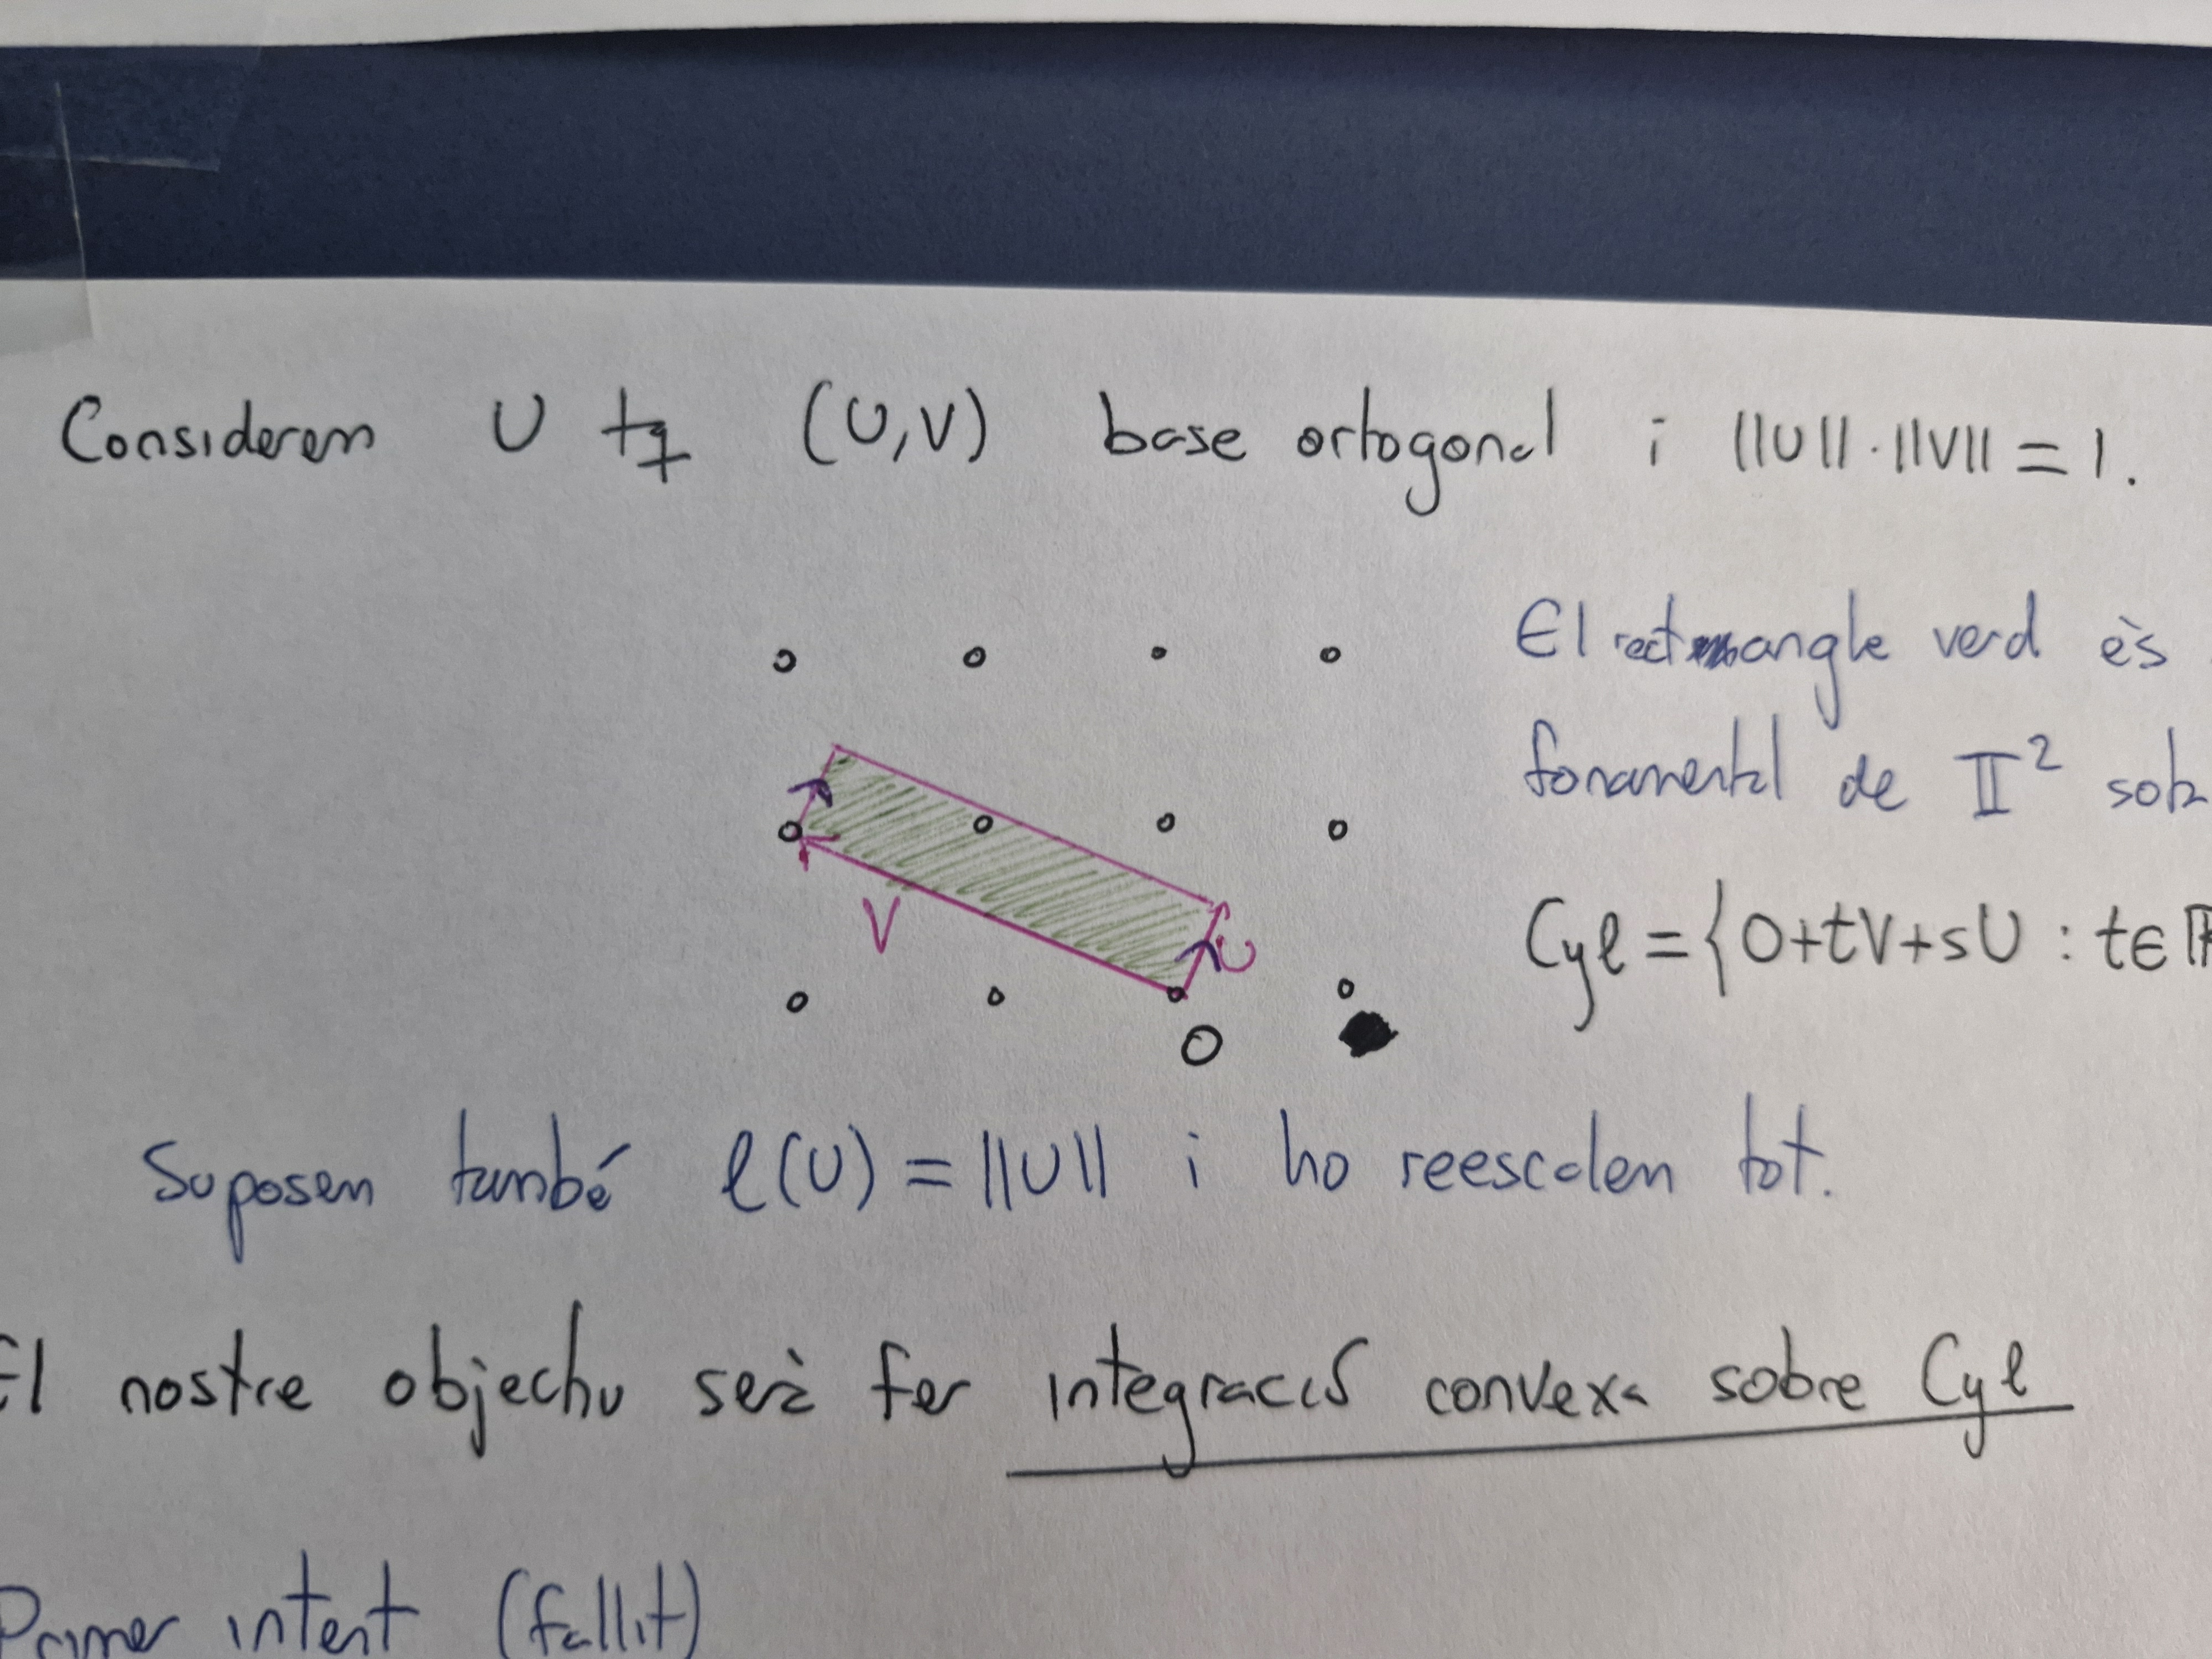
\includegraphics[width=0.5\textwidth]{Fotos/SETENA.jpg}
    \caption{{\color{blue}TEXT}}
    \label{fig:setena_foto}
\end{figure}

\subsection{Integració convexa del cilindre $\mathcal Cil$}
\begin{nota}
    En aquest capítol, denotem per $X\cdot f$ la derivada de l'aplicació $f$ al llarg del camp vectorial $X$, és a dir, $X\cdot f := \text df(X)$.
\end{nota}
Per tal de poder aplicar el lema \ref{lema:C0-1D}, no és prou amb prendre una família de corbes unidimensionals qualssevol, com
\begin{align}
    \nonumber\phi_t:[0,1]&\to\mathbb T^2\\
    \nonumber s&\mapsto [O+tV+sU],
\end{align}
sinó que haurà de ser una mica més elaborat. 

En concret, definim 
\begin{equation*}
    W=U+\zeta V, \text{ on } \zeta = -\frac{\mu(U,V)}{\mu(V,V)} = -\frac{\langle U\cdot f, V\cdot f\rangle}{\langle V\cdot f, V\cdot f\rangle}.
\end{equation*}
Observem que, amb aquesta definició, $\mu(W,V)=0$. Ara podem definir la família de corbes $\varphi(t,\cdot):[0,1]\to\mathbb \mathcal Cil$ tals que 
\begin{equation*}
    \varphi(t,0) = O + tV, \text{ i } \frac{\partial\varphi}{\partial s}(t,s) = W(\varphi(t,s)).
\end{equation*}
Resolent l'equació diferencial, obtenim
\begin{equation*}
    \varphi(t,s) = O + sU + \psi(t,s)V
\end{equation*}
per alguna funció $\psi:(\mathbb R/\mathbb Z)\times[0,1]\to\mathbb R$ amb $\psi(t,0)=t$. En particular, $\varphi(t,\cdot)$ connecta $O+tV$ i $O+U+\psi(t,1)V$. Així, $\varphi:\mathbb R/\mathbb Z\times[0,1]\to\mathcal Cil$ és un difeomorfisme. A més, 
\begin{equation*}
    \ell\left( \frac{\partial\varphi}{\partial t} \right) = 0, \text{ i } \mu\left( \frac{\partial\varphi}{\partial t}, W \right) = 0.
\end{equation*}

\begin{figure}[htbp]
    \centering
    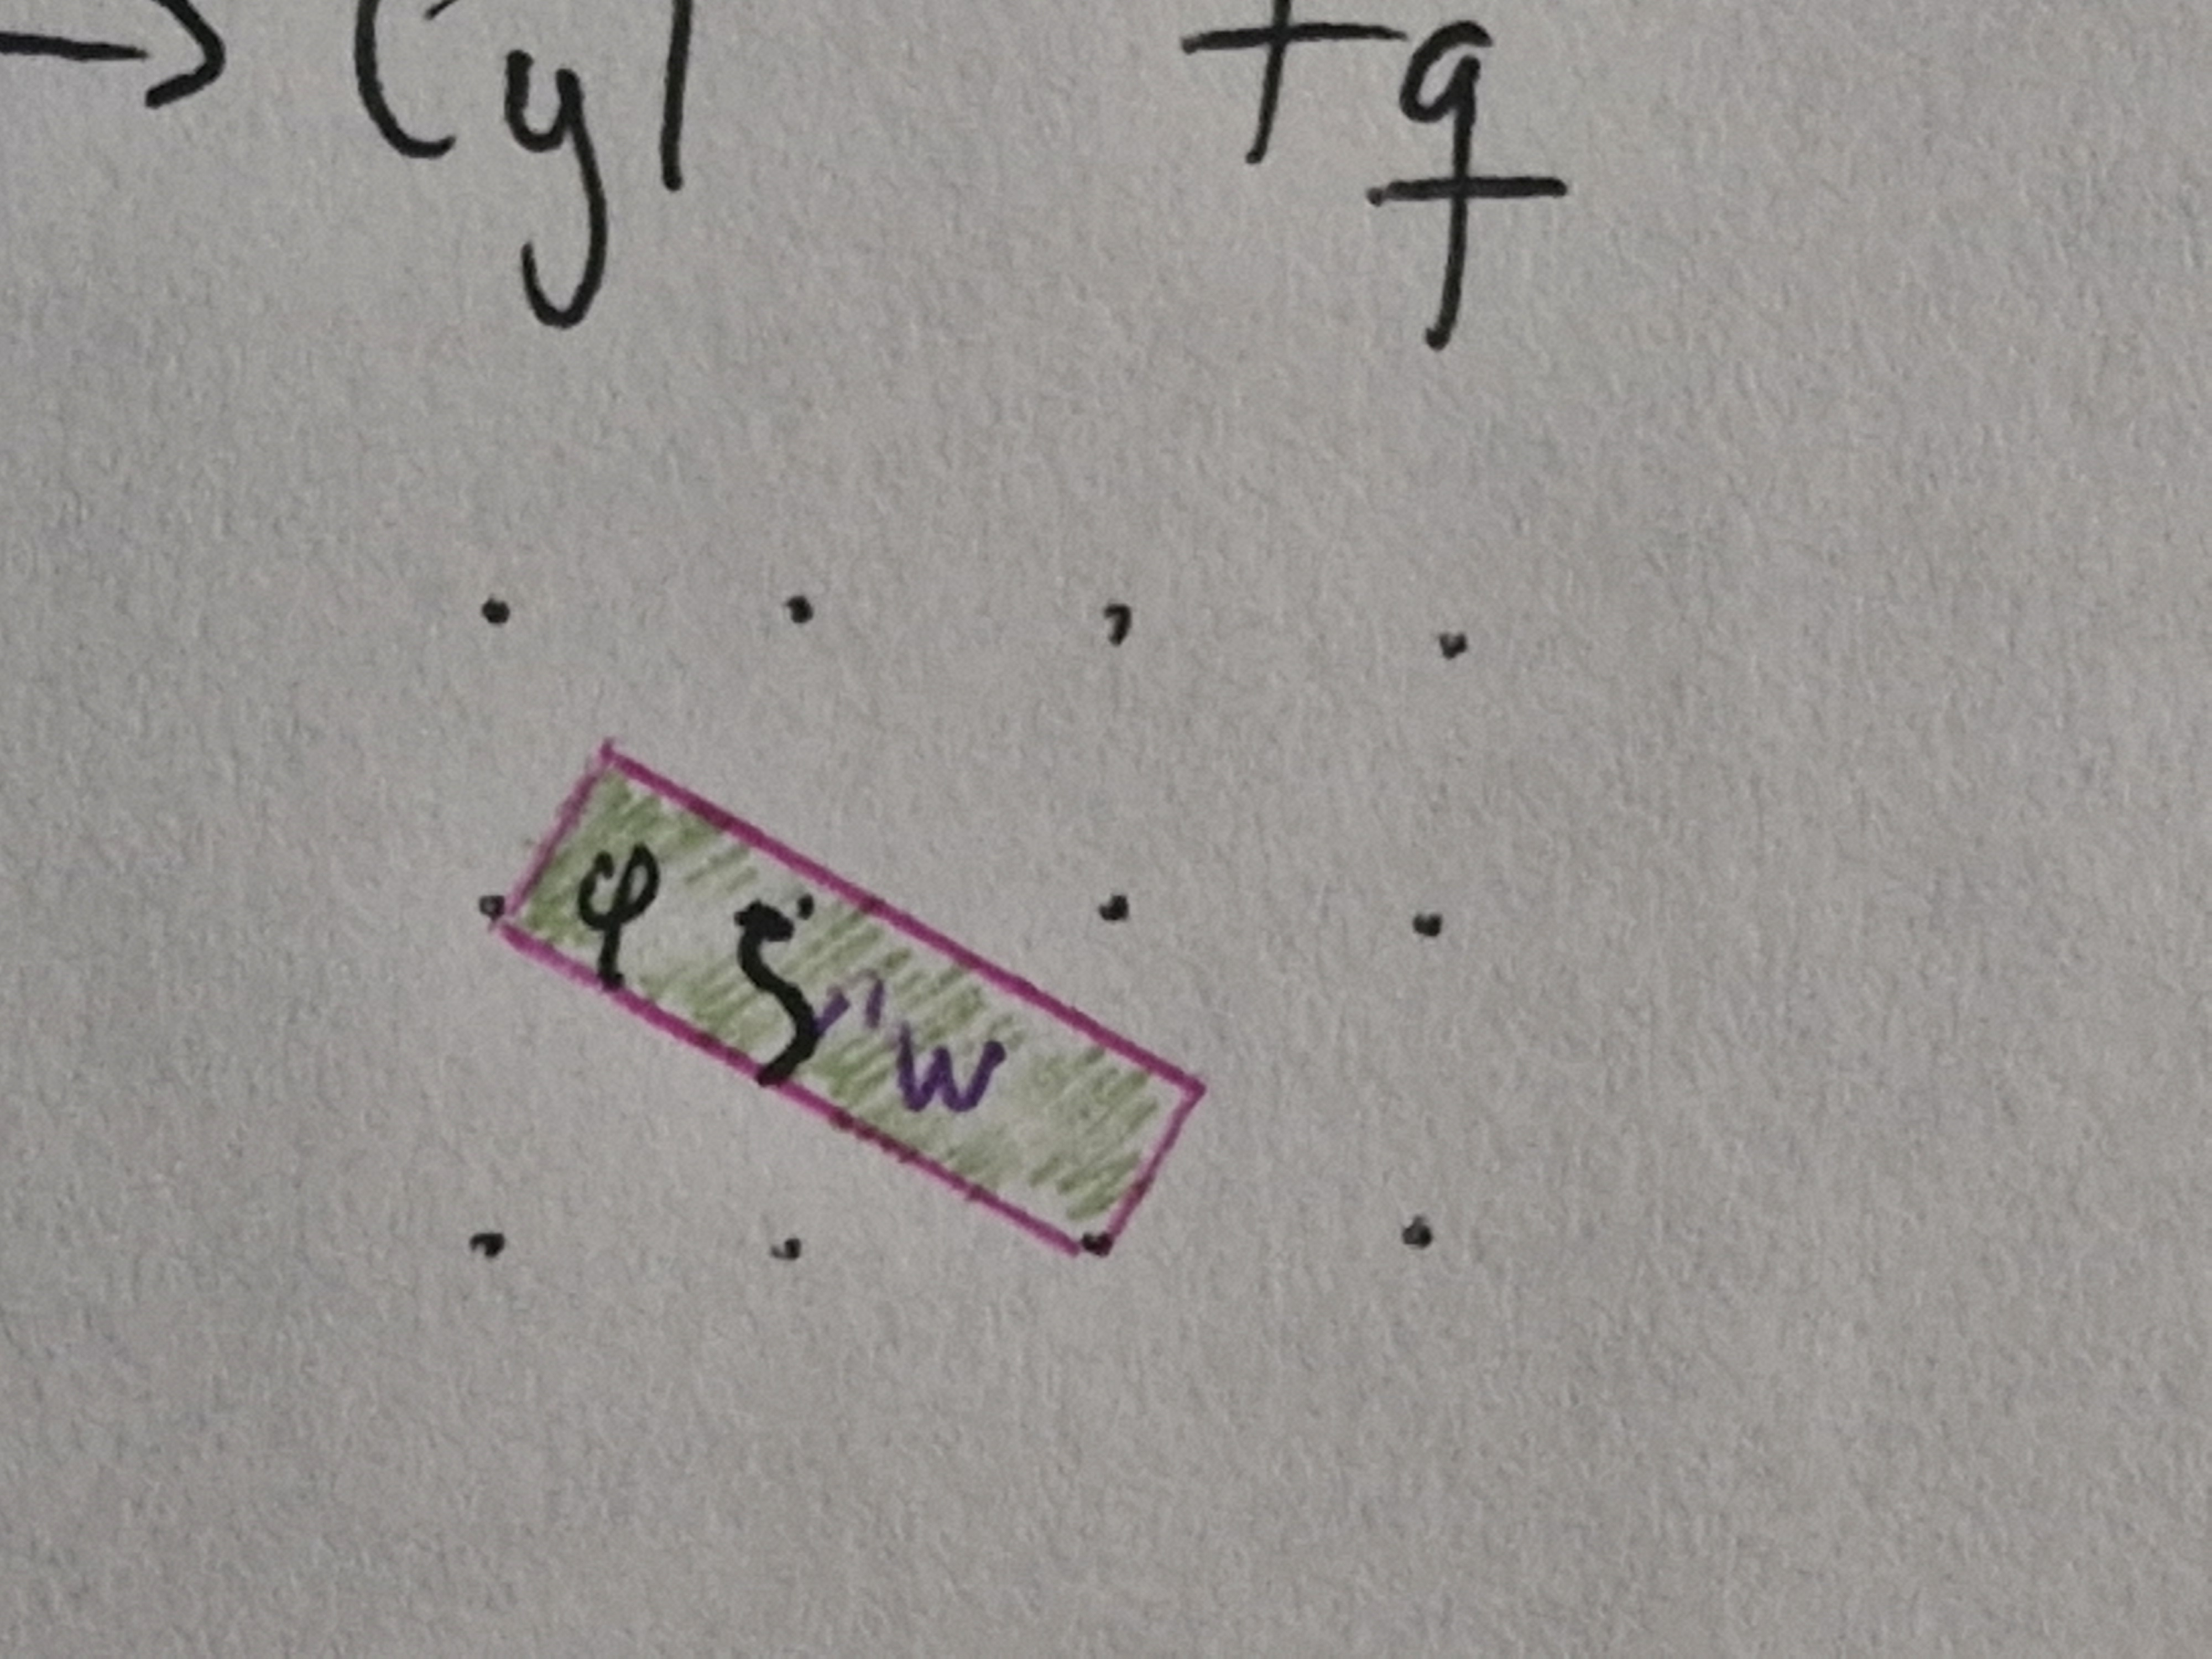
\includegraphics[width=0.5\textwidth]{Fotos/VUITENA.jpg}
    \caption{{\color{blue}TEXT}}
    \label{fig:vuitena_foto}
\end{figure}

Voldrem aplicar integració convexa a cada corba $f\circ\varphi(t,\cdot)$. Per fer-ho, considerem ara les voltes $h(t,s,u)$ donades per
\begin{equation}
    h(t,s,u) = \bar h(\varphi(t,s), \cos(2\pi u))
\end{equation}
on 
\begin{equation*}
    \bar h(p, c) = r(p)\left( \cos(\alpha(p)c)\vec t(p) + \sin(\alpha(p)c)\vec n(p) \right),
\end{equation*}
amb $r:=\sqrt{\mu(W,W)}$, $\vec t := \frac{W\cdot f}{\|W\cdot f\|}$, $\vec n := \frac{W\cdot f\times V\cdot f}{\|W\cdot f\times V\cdot f\|}$ i $\alpha:= J_0^{-1}(\|W\cdot f\|/r)$.

Si ara escrivim 
\begin{equation*}
    (W\cdot f)(\varphi(t,s)) = \frac{\partial(f\circ\varphi)}{\partial s}(t,s)= \int_0^1 h(t,s,u) du,
\end{equation*}
obtenim l'aplicació suau $F:(\mathcal Cil, \mu)\to(\mathbb R^3, \langle\cdot, \cdot\rangle)$ amb
\begin{equation}
    F\circ\varphi(t,s) := f(O+tV) + \int_0^s h(t,u,\set{Nu}) du.
\end{equation}

A continuació, enunciem alguns lemes que caracteritzaran la diferència entre $F$ i $f$ i les seves derivades.

\begin{lema}
    \label{lema:lema2}
    Siguin $f$, $h$, $N$ i $F$ com hem definit més amunt. Aleshores,
    \begin{equation*}
        \|F-f\|_{C^0} \le \frac{K(h)}{N},
    \end{equation*}
    on $K(h)$ només depèn de $\|h\|_{C^1}$.
\end{lema}

\begin{lema}
    \label{lema:lema3}
    Siguin $f$, $h$, $N$ i $F$ com hem definit més amunt. Aleshores,
    \begin{equation*}
        \left\|\frac{\partial (F\circ \varphi)}{\partial t}-\frac{\partial (f\circ \varphi)}{\partial t}\right\|_{C^0} \le \frac{K(h)}{N},
    \end{equation*}
    on $K(h)$ només depèn de $\|h\|_{C^2}$.
\end{lema}

\begin{lema}
    \label{lema:lema4}
    Siguin $f$ i $F$ com hem definit més amunt i $\mu = f^*\langle\cdot, \cdot\rangle + \rho\ell\otimes\ell$. Aleshores,
    \begin{equation*}
        \left\|W\cdot F-W\cdot f\right\|_{C^0} \le \sqrt7\cdot\|U\|\cdot\|\rho\|^{1/2}_{C^0}.
    \end{equation*}
\end{lema}

% \begin{lema}
%     {\color{blue} SI AQUEST LEMA NO ES FA SERVIR ENS EL CARREGUEM}
%     Es verifica
%     \begin{equation*}
%         1+J_0^2(\alpha)-2J_0(\alpha)\cos(\alpha) \le 7(1-J_0^2(\alpha)).
%     \end{equation*}
%     per tot $\alpha\in[0,z]$, on $z$ és el primer zero de $J_0$.
% \end{lema}

\begin{lema}
    \label{lema:lema6}
    \begin{equation*}
        \left\| \text dF -\text df \right\|_{C^0} \le \sqrt{7}\|\rho\|^{1/2}_{C^0} + \frac{K(\zeta,\psi,h)}{N}
    \end{equation*}
    on $K(\zeta,\psi,h)$ només depèn de $\|\zeta\|_{C^0}$, de $\left\|\left(  \frac{\partial\psi}{\partial t}\right)^{-1}\right\|_{C^0}$ i $\|h\|_{C^2}$.
\end{lema}

% {\color{green!50!black}
%     \textit{Prova.} Com $(U,V)$ és una base directa ortogonal, aleshores 
%     \begin{equation*}
%         \|dF-df\|\le \frac{\|U\cdot F - U\cdot f\|}{\|U\|} + \frac{\|V\cdot F - V\cdot f\|}{\|V\|}.
%     \end{equation*}
%     A més, $\frac{\partial \varphi}{\partial t} = \frac{\partial \psi}{\partial t}V$. Per tant,
%     \begin{equation}\label{eq: dospuntonze}
%         \|V\cdot F - V\cdot f\| = \left|\frac{\partial\psi}{\partial t}\right|^{-1} \left\| \frac{\partial(F\circ\varphi)}{\partial t} - \frac{\partial(f\circ\varphi)}{\partial t} \right\|.
%     \end{equation}
%     Com $W=U+\zeta V$, obtenim
%     \begin{equation*}
%         \|U\cdot F - U\cdot f\| \le \|W\cdot F - W\cdot f\| + |\zeta |\cdot\|V\cdot F - V\cdot f\|.
%     \end{equation*}
%     Per últim, prenent les últimes tres equacions,
%     \begin{equation}\label{eq:demo lema 6}
%         \|dF-df\|\le \frac{\|W\cdot F - W\cdot f\|}{\|U\|} + \frac{|\zeta|\cdot\|V\|^2+1}{\|V\|}\left|\frac{\partial\psi}{\partial t}\right|^{-1} \left\| \frac{\partial(F\circ\varphi)}{\partial t} - \frac{\partial(f\circ\varphi)}{\partial t} \right\|.
%     \end{equation}
%     Aplicant els lemes \ref{lema:lema3} i \ref{lema:lema4}, obtenim el resultat. \qed
% }
\begin{lema}
    \label{lema:lema7}
    \begin{equation*}
        \|\mu-F^*\langle\cdot, \cdot\rangle\|_{C^0} \le \frac{K(f\circ\varphi,h)}{N}\|\textrm d\varphi ^{-1}\|_{C^0}^2,
    \end{equation*}
    on $K(f\circ\varphi,h)$ només depèn de $\|\frac{\partial(f\circ\varphi)}{\partial t}\|_{C^0}$ i de $\|h\|_{C^2}$.
\end{lema}

\begin{obs}
    Observem que els lemes que acabem d'enunciar tenen una relació directa amb els lemes i proposicions que hem demostrat al capítol anterior. Si bé la pertorbació que fem és diferent a la de Nash, és evident, per exemple, que el lema \ref{lema:lema2} és equivalent a la observació que la pertorbació \eqref{eq:pertorbacio} té terme d'error $O\left(\frac{1}{\lambda}\right)$. De la mateixa manera, el lema \ref{lema:lema6} ens relaciona el canvi en primeres derivades, com en la proposició \ref{prop:primer_derivada}, i el canvi mètric del lema \ref{lema:lema7} és similar al demostrat en la proposició \ref{prop:mida_pertorbacio}.
\end{obs}


% {
% \color{green!50!black}
% \textit{Prova.} 
% Primer volem acotar la diferència entre $\varphi^*\mu$ i $\varphi^*F^*\langle\cdot, \cdot\rangle = (F\circ\varphi)^*\langle\cdot, \cdot\rangle$. Notem que 
% \begin{align*}
%     (F\circ\varphi)^*\langle\cdot, \cdot\rangle(\partial_s, \partial_s) 
%     &= \left\|\frac{\partial(F\circ\varphi)}{\partial s}\right\|^2
%     \\
%     &= \|h(t,s,\set{Ns})\|^2
%     \\
%     &= \mu(W,W)
%     \\
%     &= \varphi^*(\mu)(\partial_s, \partial_s).
% \end{align*}
% Per tant, com $\mu\left(\frac{\partial\varphi}{\partial t},\frac{\partial\varphi}{\partial t}\right) = f^*\langle\cdot, \cdot\rangle\left(\frac{\partial\varphi}{\partial t},\frac{\partial\varphi}{\partial t}\right)$, tenim que
% \begin{align*}
%     |((F\circ\varphi)^*\langle\cdot, \cdot\rangle - \varphi^*\mu)(\partial_t, \partial_t)| 
%     &= 
%     \left|
%     \left\|  \frac{\partial F\circ\varphi}{\partial t} \right\|^2 - \left\|\frac{\partial f\circ\varphi}{\partial t}\right\|
%     \right|
%     \\
%     &\le \left\|\frac{\partial F\circ\varphi}{\partial t} - \frac{\partial f\circ\varphi}{\partial t}\right\|\left\|\frac{\partial F\circ\varphi}{\partial t} - \frac{\partial f\circ\varphi}{\partial t}\right\|
%     \\
%     &\le \left\|\frac{\partial F\circ\varphi}{\partial t} - \frac{\partial f\circ\varphi}{\partial t}\right\|\left(2\left\|\frac{\partial f\circ\varphi}{\partial t}\right\|+\left\|\frac{\partial F\circ\varphi}{\partial t} - \frac{\partial f\circ\varphi}{\partial t}\right\|\right)
% \end{align*}
% De manera que, pel lema \ref{lema:lema3},
% \begin{equation*}
%     |((F\circ\varphi)^*\langle\cdot, \cdot\rangle - \varphi^*\mu)(\partial_t, \partial_t)| \le \frac{K_1(f\circ\varphi,h)}{N},
% \end{equation*}
% on $K_1(f\circ\varphi,h)$ només depèn de $\|\frac{\partial(f\circ\varphi)}{\partial t}\|_{C^0}$ i de $\|h\|_{C^2}$. 

% Per la manera en què hem definit els vectors, tenim que 
% \begin{equation*}
%     f^*\langle\cdot, \cdot\rangle\left(\frac{\partial\varphi}{\partial t},\frac{\partial\varphi}{\partial s}\right) = \mu\left(\frac{\partial\varphi}{\partial t},\frac{\partial\varphi}{\partial s}\right) = \mu\left(\frac{\partial\varphi}{\partial t},W\right) = 0,
% \end{equation*}
% d'on podem inferir que 
% \begin{equation*}
%     \left\langle \frac{\partial(f\circ\varphi)}{\partial t}, h(t,s,\set{Ns})\right\rangle = 0.
% \end{equation*}
% Per tant,
% \begin{align*}
%     |((F\circ\varphi)^*\langle\cdot,\cdot\rangle-\varphi^*\mu)(\partial_t,\partial_s)| &= |(F\circ\varphi)^*\langle\partial_t,\partial_s\rangle - \varphi^*\mu(\partial_t,\partial_s)|
%     \\
%     &= \left|\left\langle \frac{\partial(F\circ\varphi)}{\partial t}, h(t,s,\set{Ns}) \right\rangle\right|
%     \\
%     &= \left|\left\langle \frac{\partial(F\circ\varphi)}{\partial t}-\frac{\partial(f\circ\varphi)}{\partial t}, h(t,s,\set{Ns}) \right\rangle\right|
%     \\
%     &\le \left\| \frac{\partial(F\circ\varphi)}{\partial t} -\frac{\partial(f\circ\varphi)}{\partial t}\right\\||h(t,s,\set{Ns})\|.
% \end{align*}
% De manera que, de nou pel lema \ref{lema:lema3},
% \begin{equation}\label{eq:cosa_K2}
%     |((F\circ\varphi)^*\langle\cdot,\cdot\rangle-\varphi^*\mu)(\partial_t,\partial_s)| \le \frac{K_2(h)}{N},
% \end{equation}
% Tot plegat, 
% \begin{equation*}
%     \|\varphi^*\mu - \varphi^*F^*\langle\cdot,\cdot\rangle\|_{C^0} \le \frac{K_1(f\circ \varphi, h) + 2K_2(h)}{N}.
% \end{equation*}
% I acabem amb 
% \begin{equation*}
%     \|\mu-F^*\langle\cdot,\cdot\rangle\| \le \|\varphi^*\mu - \varphi^*F^*\langle\cdot,\cdot\rangle\| \|d\varphi^{-1}\|^2_{C^0}.
% \end{equation*}
% \qed
% }





    
\subsection{Integració convexa del tor $\mathbb T^2$}
Amb la integració convexa del cilindre, hem obtingut una aplicació $F:(\mathcal Cil, \mu)\to(\mathbb R^3, \langle\cdot, \cdot\rangle)$ gairebé isomètrica i $C_0$-propera a l'aplicació induïda sobre $\mathcal Cil$ per $f:(\mathbb T^2, \mu)\to(\mathbb R^3, \langle\cdot, \cdot\rangle)$. Ara bé, les imatges de les dues corbes que defineixen la frontera del cilindre no coincideixen necessàriament. Per tant, el nostre objectiu serà deformar $F$ de tal manera que coincideixin, tal que sigui possible prendre el quocient d'aquesta nova aplicació per a obtenir un encabiment isomètric del tor pla.

\begin{figure}[htbp]
    \centering
    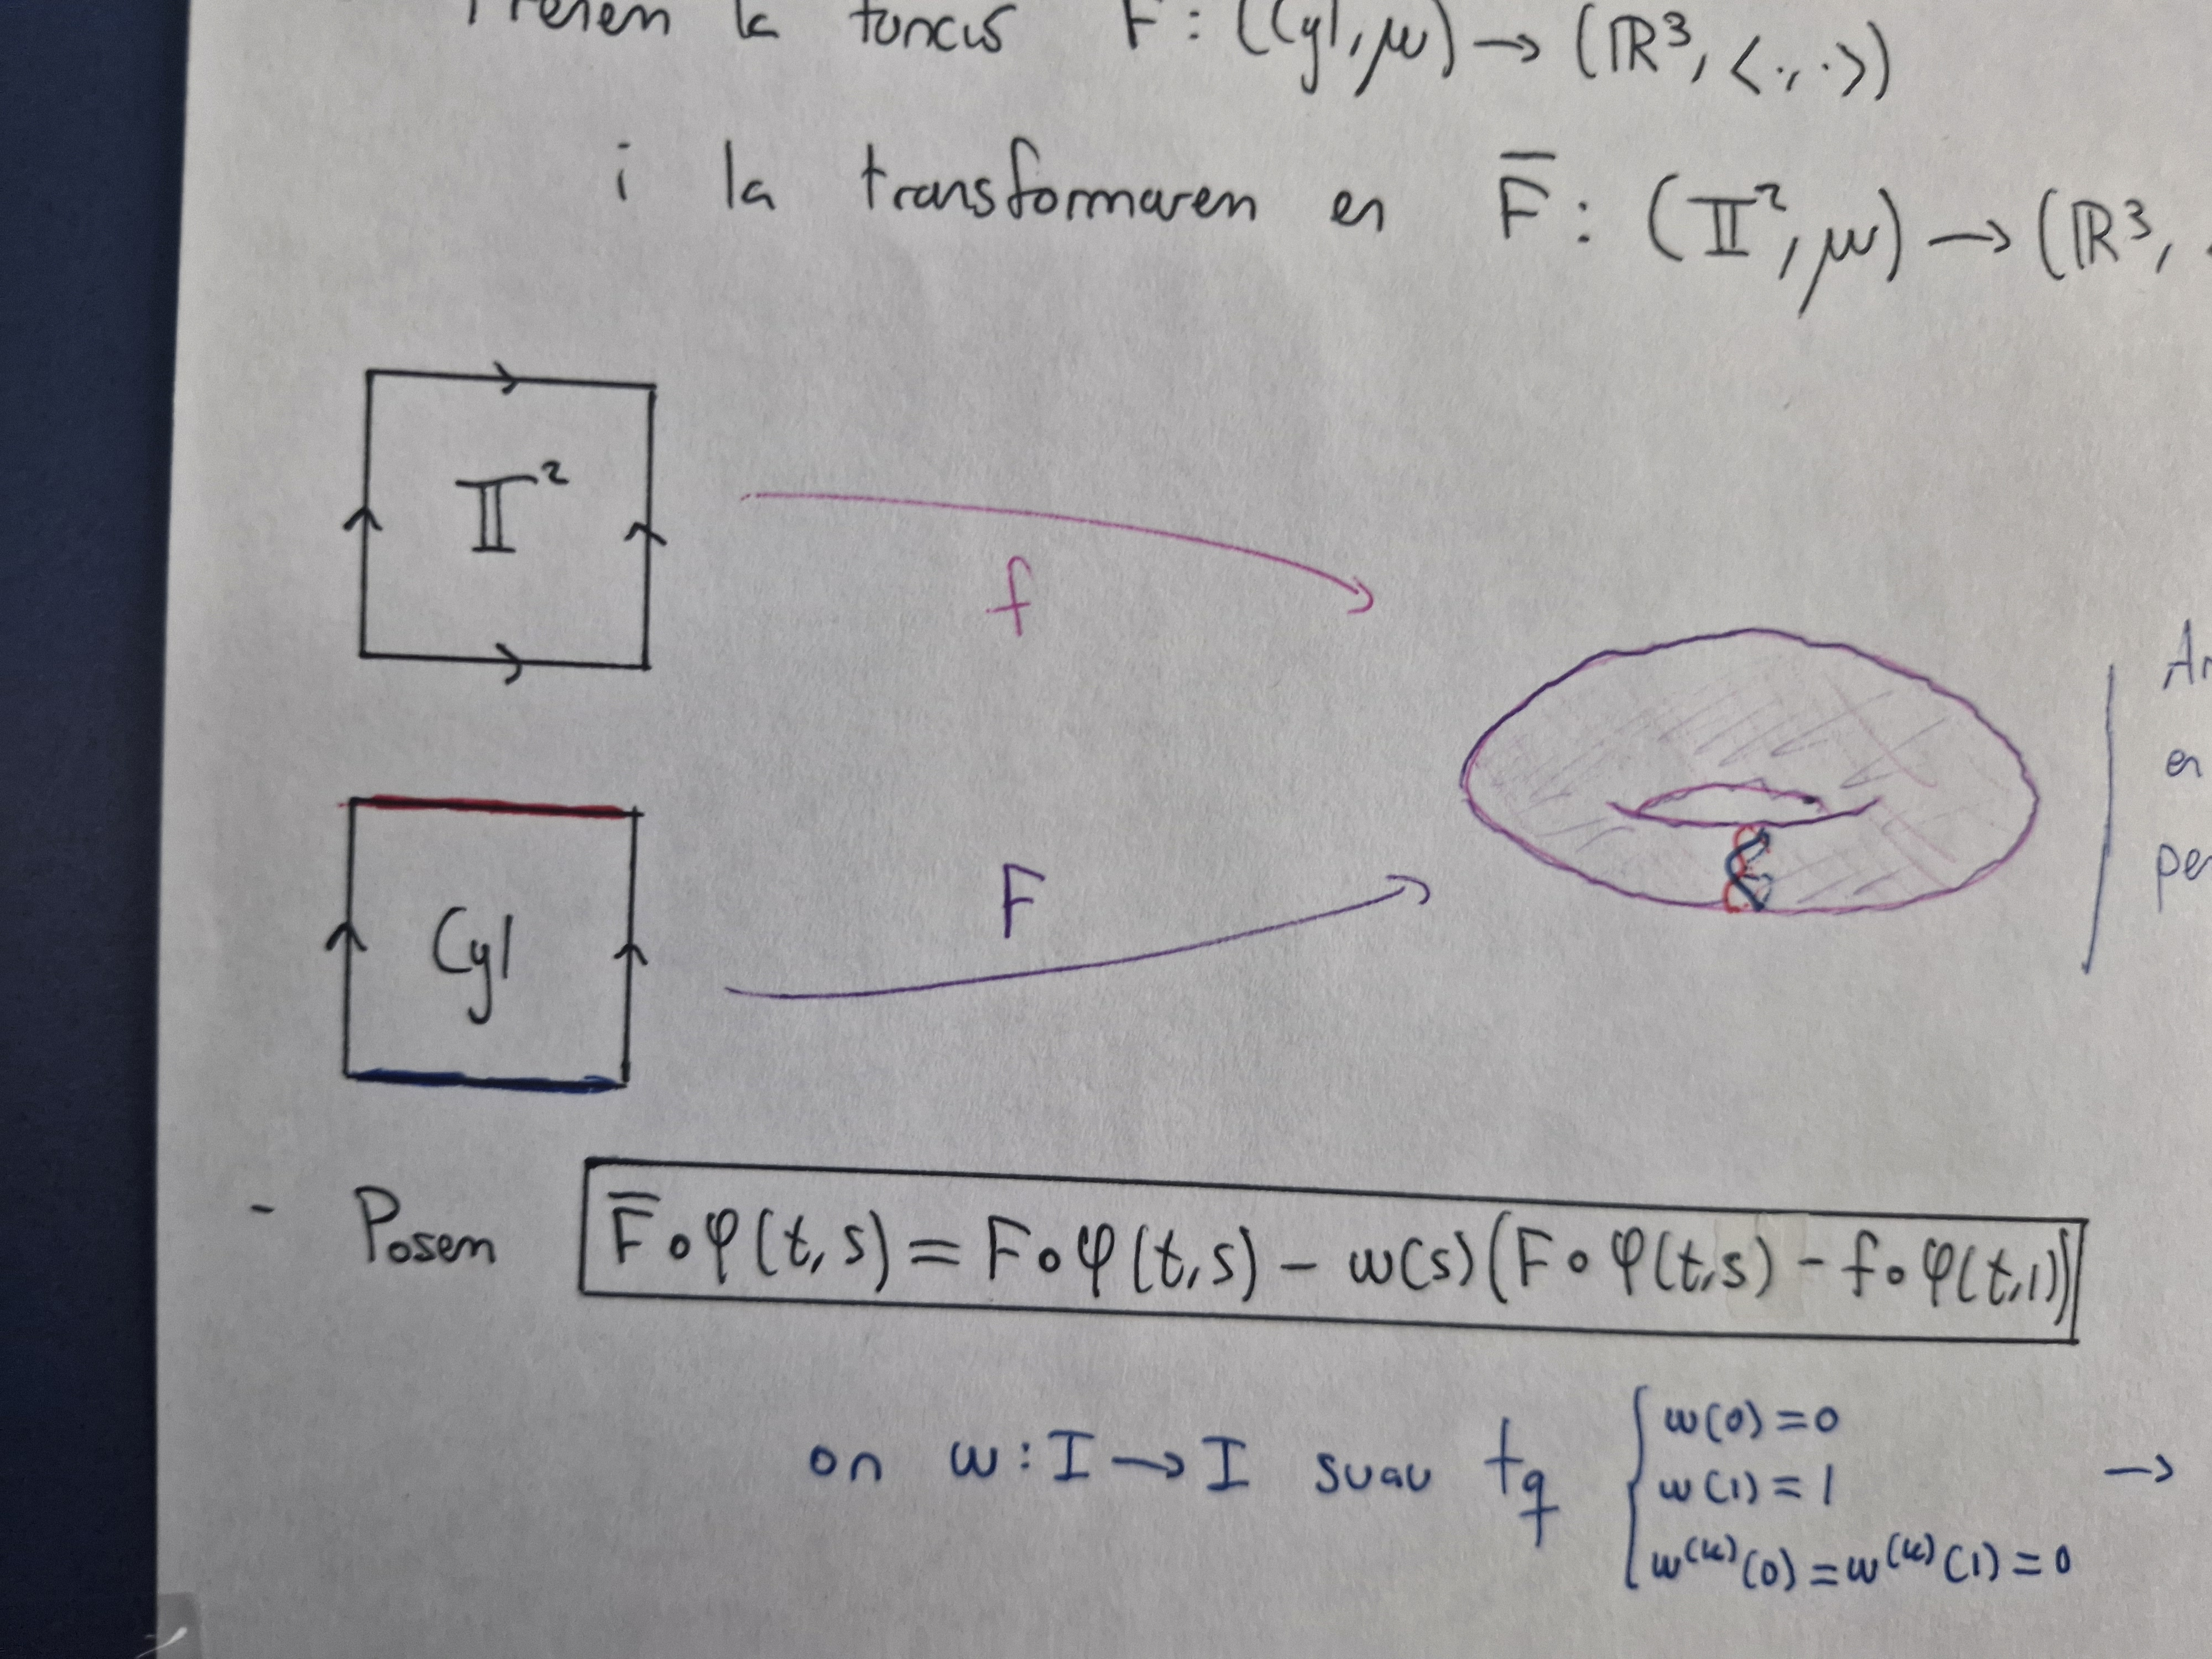
\includegraphics[width=0.5\textwidth]{Fotos/NOVENA.jpg}
    \caption{{\color{blue}TEXT}}
    \label{fig:novena_foto}
\end{figure}

Definim una nova aplicació $\bar F$ tal que
\begin{equation}
    \label{eq:def_barF}
    \bar F\circ\varphi(t,s) := F\circ\varphi(t,s) - w(s)(F\circ\varphi(t,1)-f\circ\varphi(t,1)),
\end{equation}
on $w:I\to I$ és una funció $C^\infty$ tal que 
\begin{equation*}
    w(0)=0, \text{ } w(1)=1 \text{ i } w^{(k)}(0)=w^{(k)}(1)=0.
\end{equation*}
\begin{lema}
    \label{lema:lema8}
    Si $f:\mathbb T^2\to\mathbb R^3$ i $w:I\to I$ són de classe $C^\infty$, aleshores $\bar F$ és de classe $C^\infty$ com a aplicació de $\mathbb T^2$ en $\mathbb R^3$.
\end{lema}
Podem reunir tots aquests tots els resultats que hem enunciat fins ara en el teorema següent, el \textbf{\textit{One Step Theorem}}. És evident que aquest teorema recull tots els canvis que es donen en un pas d'integració convexa, en el sentit de \textit{pas} que hem vist a la demostració del teorema de Nash.
\begin{teo}[One Step Theorem]\label{teo:OneStep}
    Sigui $f:(\mathbb T^2, \mu)\to(\mathbb R^3, \langle\cdot, \cdot\rangle)$ un encabiment de classe $C^\infty$ tal que $\mu = f^*\langle\cdot, \cdot\rangle + \rho\ell\otimes\ell$ i $\rho\in L^\infty(\mathbb T^2)$. Aleshores, 
    \begin{enumerate}
        \item $\|\bar F-f\|_{C^0}\le\frac{K_1(h)}{N}$ i $\|\bar F-f\|_{C^0}\le 2\sqrt7\|U\|\cdot\|\rho\|^{1/2}_{C^0}$,
        \item $\|\text d\bar F-\text df\|_{C^0}\le\frac{K_2(h,\zeta,\psi,w')}{N} + \sqrt7\|\rho\|^{1/2}_{C^0}$,
        \item $\|V\cdot\bar F-V\cdot f\|_{C^0}\le\frac{K_3(h,\psi)}{N}$,
        \item $\|W\cdot\bar F-W\cdot f\|_{C^0}\le\sqrt7\|U\|(1+\|w'\|_{C^0})\|\rho\|^{1/2}_{C^0}$, i
        \item $\|\mu - \bar F^*\langle\cdot, \cdot\rangle\|_{C^0}\le\frac{K_4(f\circ\varphi,r,h,w',\varphi^{-1})}{N}$.
    \end{enumerate}
    on 
    \begin{itemize}
        \item $K_1(h)$ només depèn de $\|h\|_{C^1}$.
        \item $K_2(h,\zeta,\psi,w')$ només depèn de $\|\zeta\|_{C^0}$, de $\left\|\left(  \frac{\partial\psi}{\partial t}\right)^{-1}\right\|_{C^0}$, de $\|w'\|_{C^0}$ i de $\|h\|_{C^2}$.
        \item $K_3(h,\psi)$ només depèn de $\left\|\left(  \frac{\partial\psi}{\partial t}\right)^{-1}\right\|_{C^0}$ i de $\|h\|_{C^2}$.
        \item $K_4(f\circ\varphi,r,h,w',\varphi^{-1})$ només depèn de $\|\frac{\partial(f\circ\varphi)}{\partial t}\|_{C^0}$, de $\|w'\|_{C^0}$, de $\|r\|_{C^0}$, de $\left\|\text d\varphi^{-1}\right\|_{C^0}$ i de $\|h\|_{C^2}$.
    \end{itemize}
\end{teo}
\begin{nota}
    Anomenarem 
    \begin{equation*}
        IC(f,\mu,N):=\bar F
    \end{equation*}
    l'aplicació obtinguda amb un pas d'integració convexa de l'aplicació $f$, la mètrica $\mu$ i el nombre d'oscil·lació $N$.
\end{nota}
% {
%     \color{green!50!black}
%     \textit{Prova.}

%     \underline{Primer punt.}
%     De la definició \eqref{eq:def_barF}, tenim que
%     \begin{equation}\label{eq: 2Ff}
%         \|\bar F(p)-f(p)\|\le\|F(p)-f(p)\| + \|w(s)\|_{C^0} \|F-f\|_{C^0} \le 2\|F-f\|_{C^0}.
%     \end{equation}
%     Pel lema \ref{lema:lema2}, $\|F-f\|_{C^0}\le\frac{K(h)}{N}$. Així, obtenim la primera desigualtat del primer punt del teorema,
%     \begin{equation*}
%         \|\bar F(p)-f(p)\|_{C^0}\le\frac{K_1(h)}{N}.
%     \end{equation*}
%     Per la segona desigualtat, considerem
%     \begin{align*}
%         \|F\circ\varphi(t,s)-f\circ\varphi(t,s)\| &= \left\|\int_0^s \left( \frac{\partial F\circ\varphi}{\partial s}(t,u) -  \frac{\partial f\circ\varphi}{\partial s}(t,u)\right)\text du\right\|\\
%         &\le \int_0^s\left\| 
%             (W\cdot F)(\varphi(t,u)) - (W\cdot f)(\varphi(t,u))
%         \right\|\text du\\
%         &\le \|W\cdot F-W\cdot f\|_{C^0}.
%     \end{align*}
%     Pel lema \ref{lema:lema4}, $\|W\cdot F-W\cdot f\|_{C^0}\le\sqrt7\|U\|\cdot\|\rho\|^{1/2}_{C^0}$. Prenent això i la desigualtat \eqref{eq: 2Ff}, obtenim la segona desigualtat del primer punt del teorema,
%     \begin{equation*}
%         \|\bar F-f\|_{C^0}\le 2\sqrt7\|U\|\cdot\|\rho\|^{1/2}_{C^0}.
%     \end{equation*}

%     \underline{Segon punt.}
%     Seguim la demostració del lema \ref{lema:lema6} per a obtenir una desigualtat anàloga a \eqref{eq:demo lema 6},
%     \begin{equation*}
%         \|d\bar F-df\|\le \frac{\|W\cdot\bar F - W\cdot f\|}{\|U\|} + \frac{|\zeta|\cdot\|V\|^2+1}{\|V\|}\left|\frac{\partial\psi}{\partial t}\right|^{-1} \left\| \frac{\partial(\bar F\circ\varphi)}{\partial t} - \frac{\partial(f\circ\varphi)}{\partial t} \right\|.
%     \end{equation*}
%     Derivant la definició \eqref{eq:def_barF} respecte de $t$ i $s$, obtenim les desigualtats
%     \begin{equation}\label{eq: respecte t}
%         \|W\cdot\bar F - W\cdot f\| \le \|W\cdot F - W\cdot f\|_{C^0} + \|w'\|_{C^0}\|F - f\|_{C^0}.
%     \end{equation}
%     \begin{equation}\label{eq: respecte s}
%         \left\| \frac{\partial(\bar F\circ\varphi)}{\partial t} - \frac{\partial(f\circ\varphi)}{\partial t} \right\| \le 2\left\| \frac{\partial(F\circ\varphi)}{\partial t} - \frac{\partial(f\circ\varphi)}{\partial t} \right\|_{C^0}
%     \end{equation}
%     Prenent aquestes tres desigualtats, 
%     \begin{align*}
%         \|d\bar F-df\|_{C^0}
%         &\le\frac{1}{\|U\|}\left(\|W\cdot F - W\cdot f\|_{C^0} + \|w'\|_{C^0}\|F - f\|_{C^0}\right) 
%         \\&\quad\quad\quad+ \frac{|\zeta|\cdot\|V\|^2+1}{\|V\|}\left|\frac{\partial\psi}{\partial t}\right|^{-1}\left( 2\left\| \frac{\partial(F\circ\varphi)}{\partial t} - \frac{\partial(f\circ\varphi)}{\partial t} \right\|_{C^0}\right),
%     \end{align*}
%     i amb els lemes \ref{lema:lema2}, \ref{lema:lema3} i \ref{lema:lema4}, obtenim la desigualtat del segon punt del teorema.

%     \underline{Tercer punt.}
%     Prenent una equació com la de \eqref{eq: dospuntonze} i considerant la desigualtat obtinguda derivant respecte de $s$, \eqref{eq: respecte s}, trobem
%     \begin{align*}
%         \|V\cdot \bar F - V\cdot f\| &= \left|\frac{\partial\psi}{\partial t}\right|^{-1} \left\| \frac{\partial(\bar F\circ\varphi)}{\partial t} - \frac{\partial(f\circ\varphi)}{\partial t} \right\|\\
%         &\le 2\left|\frac{\partial\psi}{\partial t}\right|^{-1} \left\| \frac{\partial(F\circ\varphi)}{\partial t} - \frac{\partial(f\circ\varphi)}{\partial t} \right\|_{C^0}.
%     \end{align*}
%     aplicant el lema \ref{lema:lema3}, obtenim el tercer punt del teorema.

%     \underline{Quart punt.}
%     Prenent la desigualtat obtinguda derivant respecte de $t$, \eqref{eq: respecte t}, i considerant que $\|F-f\|_{C^0}\le\|W\cdot F - W\cdot f\|_{C^0}$, obtenim
%     \begin{equation*}
%         \|W\cdot\bar F - W\cdot f\|_{C^0}\le \|W\cdot F - W\cdot f\|_{C^0} + \|w'\|_{C^0}\|W\cdot F - W\cdot f\|_{C^0}.
%     \end{equation*}
%     Pel lema \ref{lema:lema4}, $\|W\cdot F - W\cdot f\|_{C^0}\le\sqrt7\|U\|\cdot\|\rho\|^{1/2}_{C^0}$, de manera que
%     \begin{equation*}
%         \|W\cdot\bar F - W\cdot f\|_{C^0}\le\sqrt7\|U\|\cdot\|\rho\|^{1/2}_{C^0}(1+\|w'\|_{C^0}),
%     \end{equation*}
%     tal com volíem.

%     \underline{Cinquè punt.} 
%     Seguim la demostració del lema \ref{lema:lema7} per acotar la diferència entre $\varphi^*\mu$ i $(F\circ\varphi)^*\langle\cdot,\cdot\rangle$. Per la definició \eqref{eq:def_barF}, tenim que
%     \begin{equation*}
%         (\bar F\circ\varphi)^*\langle\cdot,\cdot\rangle (\partial_s, \partial_s) = \left\|\frac{\partial(\bar F\circ\varphi)}{\partial s}\right\|^2 = \left\| W\cdot F - w'(s)(F\circ\varphi(t,1)-f\circ\varphi(t,1)) \right\|^2,
%     \end{equation*}
%     i com $\varphi^*\mu(\partial_s,\partial_s) = \|W\cdot F\|^2 = r^2$, obtenim
%     \begin{equation*}
%         |(\bar F\circ\varphi)^*\langle\cdot,\cdot\rangle(\partial_s, \partial_s) - \varphi^*\mu(\partial_s, \partial_s)| \le \|w'\|_{C^0}\|F-f\|_{C^0}(2\|r\|_{C^0} + \|w'\|_{C^0}\|F-f\|_{C^0}).
%     \end{equation*}
%     Pel lema \ref{lema:lema2}, obtenim
%     \begin{equation}\label{eq:X}
%         |(\bar F\circ\varphi)^*\langle\cdot,\cdot\rangle(\partial_s, \partial_s) - \varphi^*\mu(\partial_s, \partial_s)| \le \frac{X(w',r,h)}{N}
%     \end{equation}
%     on $X(w',r,h)$ depèn de $\|w'\|_{C^0}$, $\|r\|_{C^0}$ i $\|h\|_{C^2}$.

%     Ara, com $\varphi^*\mu(\partial_t,\partial_t) = \left\| \frac{\partial f\circ\varphi}{\partial t} \right\|^2$, obtenim
%     \begin{align*}
%         |(\bar F\circ\varphi)^*\langle\cdot,\cdot\rangle(\partial_t, \partial_t) - \varphi^*\mu(\partial_t, \partial_t)| &\le 
%         \Bigg|\left\|\frac{\partial F\circ\varphi}{\partial t}-w(s)\left(\frac{\partial F\circ\varphi}{\partial t}(t,1) - \frac{\partial f\circ\varphi}{\partial t}(t,1)\right)\right\|^2 \\&\quad\quad\quad- \left\| \frac{\partial f\circ\varphi}{\partial t} \right\|^2\Bigg|
%     \end{align*}
%     Podem escriure $A:=\frac{\partial F\circ\varphi}{\partial t}$, $B:=\frac{\partial F\circ \varphi}{\partial t}(t,1) - \frac{\partial f\circ\varphi}{\partial t}(t,1)$ i $C:=\frac{\partial f\circ\varphi}{\partial t}$.
%     \begin{align*}
%         |(\bar F\circ\varphi)^*\langle\cdot,\cdot\rangle(\partial_t, \partial_t) - \varphi^*\mu(\partial_t, \partial_t)| 
%         &=
%         \left\|\left|A-w(s)B\right\|^2 - \left\|C\right\|^2\right|
%         \\&\le
%         \left\|A-w(s)B - C\right\|\left\|A-w(s)B + C\right\|
%         \\&\le
%         (\left\|A - C\right\| + \left\|B\right\|)(\left\|A-C\right\| + 2\left\|C\right\|+\left\|B\right\|),
%     \end{align*}
%     així,
%     \begin{align*}
%         |(\bar F\circ\varphi)^*\langle\cdot,\cdot\rangle(\partial_t, \partial_t) - \varphi^*\mu(\partial_t, \partial_t)| \le 
%         4&\left\|\frac{\partial F\circ\varphi}{\partial t}-\frac{\partial f\circ\varphi}{\partial t}\right\|_{C^0}\cdot\\
%         &\left(\left\|\frac{\partial F\circ\varphi}{\partial t}-\frac{\partial f\circ\varphi}{\partial t}\right\|_{C^0}+\left\|\frac{\partial f\circ\varphi}{\partial t}\right\|_{C^0}\right).
%     \end{align*}

%     Ara pel lema \ref{lema:lema3}, tenim que 
%     \begin{equation}\label{eq:Y}
%         \left|(\bar F\circ\varphi)^*\langle\cdot,\cdot\rangle(\partial_t, \partial_t) - \varphi^*\mu(\partial_t, \partial_t)\right|\le\frac{Y(f\circ\varphi,h)}{N},
%     \end{equation}
%     on $Y(f\circ\varphi,h)$ depèn de $\|\frac{\partial(f\circ\varphi)}{\partial t}\|_{C^0}$ i de $\|h\|_{C^2}$.

%     Com $\varphi^*\mu(\partial_t,\partial_s) = \mu(\frac{\partial\varphi}{\partial t}, W)=0$, tenim
%     \begin{equation*}
%         \left|(\bar F\circ\varphi)^*\langle\cdot,\cdot\rangle(\partial_t, \partial_s) - \varphi^*\mu(\partial_t, \partial_s)\right| = \left| (\bar F\circ\varphi)^*\langle\cdot,\cdot\rangle(\partial_t, \partial_s) \right|
%     \end{equation*}

%     Posant $D=\frac{\partial F\circ\varphi}{\partial s}$, $E=F\circ\varphi(t,1) - f\circ\varphi(t,1)$ amb la notació anterior, tenim
%     \begin{align*}
%         \left|(\bar F\circ\varphi)^*\langle\cdot,\cdot\rangle(\partial_t, \partial_s)\right| &= \left|\langle A-wB, D-w'E \rangle\right|\\
%         &\le |\langle A, D\rangle| + |w'|\|E\|(\|A\| + \|B\|) + \|B\|\|D\|.
%     \end{align*}

%     Notem que $\langle A, D\rangle = (F\circ\varphi)^*\langle\cdot,\cdot\rangle(\partial_t,\partial_s)$, de manera que, per la desigualtat \eqref{eq:cosa_K2}, $|\langle A, D\rangle|\le\frac{Z_1(h)}{N}$ per alguna $Z_1$ que només depèn de $\|h\|_{C^2}$. Pel lema \ref{lema:lema2}, $\|E\|\le\frac{Z_2(h)}{N}$ per alguna $Z_2$ que només depèn de $\|h\|_{C^1}$. A més, pel lema \ref{lema:lema3}, $\|B\|\le\|A-C\|_{C^0}\le\frac{Z_3(h)}{N}$ per alguna $Z_3$ que només depèn de $\|h\|_{C^2}$. Notant que $\|A\|\le\|A-C\|+\|C\|$, obtenim $\|A\|\le\frac{Z_3(h)}{N}+\|C\|$. A més, notem que $\|D\| = \|W\cdot F\| = r$. Tot junt, obtenim
%     \begin{equation}\label{eq:Z}
%         \left|(\bar F\circ\varphi)^*\langle\cdot,\cdot\rangle(\partial_t, \partial_s)-\varphi^*\mu(\partial_t, \partial_s)\right|\le\frac{Z(f\circ\varphi,w',r,h)}{N},
%     \end{equation}
%     on 
%     \begin{equation*}
%         Z(f\circ\varphi,w',r,h) = Z_1(h) + \|w'\|_{C^0} Z_2(h)\left( \left\|\frac{\partial(f\circ\varphi)}{\partial t}\right\|_{C^0} + 2\frac{Z_3(h)}{N} \right) + Z_3(h)r.
%     \end{equation*}

%     Ara, com en la demostració del lema \ref{lema:lema7}, tenim que 
%     \begin{equation*}
%         \|\mu-\bar F^*\langle\cdot,\cdot\rangle\|\le\|\varphi^*\mu-\varphi^*\bar F^*\langle\cdot,\cdot\rangle\|\cdot\|d\varphi^{-1}\|_{C^0}.
%     \end{equation*}

%     Amb aquesta última desigualtat i les desigualtats \eqref{eq:X}, \eqref{eq:Y} i \eqref{eq:Z}, resolem el quart punt del teorema amb 
%     \begin{equation*}
%         K_4(f\circ\varphi,r,h,w',\varphi^{-1}) = (X(w',r,h) + Y(f\circ\varphi,h) + 2Z(f\circ\varphi,w',r,h))\|d\varphi^{-1}\|^2_{C^0}.
%     \end{equation*}
%     \qed
% }

\section{Encabiment isomètric del tor pla}
\begin{nota}
    En la secció anterior feiem servir $\mu$ per denotar una mètrica primitiva. Ara denotem $g$ la mètrica plana sobre el tor.
\end{nota}

A la secció anterior ens hem fixat en el cas primitiu, de manera que podíem construir una aplicació gairebé isomètrica $\bar f:(\mathbb T^2, g)\to(\mathbb R^3, \langle\cdot, \cdot\rangle)$ a partir d'una immersió $f:\mathbb T^2\to\mathbb R^3$ quan
\begin{equation*}
    g - f^*\langle\cdot, \cdot\rangle = \rho\ell\otimes\ell.
\end{equation*}

A continuació, prendrem aquests mètode i el generalitzarem al cas en què el defecte isomètric (en anglès, \textit{isometric default}) 
\begin{equation*}
    D:=g-f^*\langle\cdot, \cdot\rangle
\end{equation*}
és una mètrica. Aquest és el cas si i només si la immersió $f$ és estrictament curta. Per tal d'aplicar els resultats anteriors, haurem de descompondre aquest defecte isomètric en una suma de mètriques primitives. Observem que el conjunt de productes interiors en $\mathbb R^2$ és un con convex
\begin{equation*}
    Q_+ = \set{E\text dx\otimes\text dx + F(\text dx\otimes\text dy + \text dy\otimes\text dx) + G\text dy\otimes\text dy : EG-F^2>0, E>0, G>0}.
\end{equation*}
Per tant, podem trobar una descomposició del defecte isomètric
\begin{equation*}
    D = \sum_{j=1}^N \rho_j(D) \ell_j\otimes\ell_j,
\end{equation*}
on $N$ és un enter i les $\ell_j$ es defineixen per entorns compactes, en general.
\begin{obs}
    Observem que aquesta descomposició és l'equivalent tridimensional de la descomposició de la mètrica en formes bilinears simètriques que hem vist a la demostració de l'equació \eqref{eq:lema_descomp} al capítol anterior.
\end{obs}

El procés d'integració convexa que es presenta aquí aconsegueix trobar tres formes lineals $\ell_1, \ell_2, \ell_3$ que funcionen a un nivell global, de manera que $N$ es redueix a $3$ i no cal separar en entorns compactes.

\begin{obs}
    Aquest és el fet que simplifica enormement el càlcul de l'encabiment isomètric de \cite{borrelli2013}, ja que no cal utilitzar tota la maquinària de descomposició en entorns $\set{N_p}_p$ que hem vist a la demostració del teorema de Nash.
\end{obs}

En efecte, suposarem que la immersió $f$ és tal que el defecte isomètric pertany al con obert
\begin{equation*}
    \mathcal C:=\set{\rho_1\ell_1\otimes\ell_1 + \rho_2\ell_2\otimes\ell_2 + \rho_3\ell_3\otimes\ell_3 : \rho_1, \rho_2, \rho_3 > 0},
\end{equation*}
on $\ell_1, \ell_2, \ell_3$ són formes lineals en $\mathbb R^2$ donades per 
\begin{equation*}
    \ell_1:=\text dx, \text{ } \ell_2:=\frac{1}{\sqrt5}(\text dx + 2\text dy) \text{ i } \ell_3:=\frac{1}{\sqrt5}(\text dx - 2\text dy).
\end{equation*}
Per reduir els tres coeficients del defecte isomètric, farem tres integracions convexes, és a dir, tres passos successius. En efecte, prendrem primer
\begin{equation*}
    \mu_1 = f^*\langle\cdot, \cdot\rangle + \rho_1(D_1)\ell_1\otimes\ell_1,
\end{equation*}
amb $D_1:=D$ i construirem $f_1:=IC(f, \mu_1, N_1)$. Després, prendrem el nou defecte isomètric $D_2 := g-f_1^*\langle\cdot, \cdot\rangle\in\mathcal C$ i la mètrica
\begin{equation*}
    \mu_2 = f_1^*\langle\cdot, \cdot\rangle + \rho_2(D_2)\ell_2\otimes\ell_2,
\end{equation*}
 per obtenir $f_2:=IC(f_1, \mu_2, N_2)$. Finalment, prendrem el nou defecte isomètric $D_3 := g-f_2^*\langle\cdot, \cdot\rangle\in\mathcal C$ i la mètrica
\begin{equation*}
    \mu_3 = f_2^*\langle\cdot, \cdot\rangle + \rho_3(D_3)\ell_3\otimes\ell_3,
\end{equation*}
per obtenir $f_3:=IC(f_2, \mu_3, N_3)$. Per tal que aquests tres passos d'integració convexa resultin en un encabiment isomètric, tal com volem, haurem de veure que podem triar les constants $N_1, N_2, N_3$ prou grans tal que, després de la $i$-èssima integració convexa, el component $\rho_i$ del nou defecte isomètric sigui proper a zero, mentre la resta romanen aproximadament iguals. 

Per tal d'obtenir un encabiment isomètric, no és prou amb triar $N_1, N_2, N_3$ prou grans, sinó que caldrà repetir el procés sencer indefinidament. La realització d'aquests tres passos s'anomena, com en la demostració dels teoremes de Nash, una \textbf{etapa} (\textit{stage}). Al final de cadascuna obtenim un encabiment $\mathcal F_k$ amb una mètrica $g_k$ que és cada vegada més propera a $\langle\cdot, \cdot\rangle$. Anomenem a l'encabiment obtingut després de l'etapa $k$-èssima 
\begin{equation*}
    \mathcal F_k:=IC(\mathcal F_{k-1}, g_k, N_{k,1}, N_{k,2}, N_{k,3}),
\end{equation*}
on $\mathcal F_0:=f$. En cada etapa, ens haurem de preocupar de que el defecte isomètric $D_k:=g-f_{k-1}^*\langle\cdot, \cdot\rangle$ pertanyi al con convex $\mathcal C$.

\begin{teo}[Stage Theorem]\label{teo:Stage}
    Siguin $g$ i $\bar g$ dues mètriques Riemannianes sobre $\mathbb T^2$ i sigui 
    \begin{equation*}
        f:(\mathbb T^2, g)\to\mathbb E^3
    \end{equation*}
    una immersió tal que
    \begin{enumerate}
        \item $\bar g - g\in C^\infty(\mathbb T^2, \mathcal C)$
        \item $g-f^*\langle\cdot, \cdot\rangle\in C^\infty(\mathbb T^2, \mathcal C)$
    \end{enumerate}
    Aleshores, existeixen enters $N_1, N_2, N_3$ tals que l'immersió
    \begin{equation*}
        \bar f:=IC(f, g, N_1, N_2, N_3)
    \end{equation*}
    satisfà
    \begin{enumerate}
        \item $\bar f(0,0) = f(0,0)$
        \item $\bar g - \bar f^*\langle\cdot, \cdot\rangle\in C^\infty(\mathbb T^2, \mathcal C)$
        \item $\|\bar g - \bar f^*\langle\cdot, \cdot\rangle\|_{C^0}\le \|\bar g - g\|_{C^0}$
        \item $\|d\bar f - df\|_{C^0}\le11\|g-f^*\langle\cdot, \cdot\rangle\|_{C^0}^{\frac{1}{2}}$
    \end{enumerate}
\end{teo}

\begin{obs}
    No donarem aquí la demostració d'aquest teorema, de la mateixa manera que no n'hem conat cap en aquest capítol. Tanmateix, notem que la demostració d'aquest teorema es redueix a aplicar el teorema \ref{teo:OneStep} tres vegades, escollint $N_1, N_2, N_3$ de manera adequada per tal de minimitzar l'error i garantir que el defecte isomètric sigui proper a zero. És, per tant, similar a la demostració del teorema de Nash a l'hora de triar $\lambda$ per obtenir els $B_1, B_2, B_3$ adequats, si bé és més senzilla pel fet que no cal dividir la varietat en entorns compactes.
\end{obs}

% \subsection{Demostració del teorema \ref{teo:Stage}}
% Definim 
% \begin{equation*}
%     U(1):=\partial_x, \text{ } U(2):=\frac15(\partial_x+2\partial_y), \text{ } U(3):=\frac15(\partial_x-2\partial_y),
% \end{equation*}
% i 
% \begin{equation*}
%     V(1):=\partial_y, \text{ } V(2):=-2\partial_x+\partial_y, \text{ } V(3):=2\partial_x+\partial_y.
% \end{equation*}
% \begin{lema}
%     Sigui $B:=\rho_1\ell_1\otimes\ell_1 + \rho_2\ell_2\otimes\ell_2 + \rho_3\ell_3\otimes\ell_3$ una forma bilineal simètrica {\color{blue} definició?}. Aleshores,
%     \begin{equation*}
%         \max\set{|\rho_1|, |\rho_2|, |\rho_3|} \le \frac{5\sqrt3}8 \|B\|
%     \end{equation*}
% \end{lema}
\subsection{La successió d'immersions}
Acabem aquesta secció amb l'aplicació concreta del teorema \ref{teo:Stage} al cas del tor pla que ens interessa, de tal manera que obtindrem finalment una immersió isomètrica.

Sigui $\mathcal F_0:\mathbb T^2\to\mathbb R^3$ una immersió tal que
\begin{equation*}
    \Delta := \langle\cdot, \cdot\rangle_{\mathbb R^2} - \mathcal F_0^*\langle\cdot, \cdot\rangle\in C^\infty(\mathbb T^2, \mathcal C).
\end{equation*}
Un encabiment clàssic del tor com el de l'exemple \ref{ex:tor} amb $R$ i $r$ adequats satisfà aquesta condició. Sigui $\set{\delta_k}_k$ una successió de nombres reals positius monòtona creixent que tendeix a 1. Podem considerar una successió creixent de mètriques
\begin{equation*}
    g_k := \mathcal F_0^*\langle\cdot, \cdot\rangle + \delta_k\Delta.
\end{equation*}
que convergeix a la mètrica plana en el tor. Podem construir una successió d'immersions
\begin{equation*}
    \mathcal F_k := IC(\mathcal F_{k-1}, g_k, N_1, N_2, N_3)
\end{equation*}
aplicant el teorema \ref{teo:Stage} per a cada $k\in\mathbb N$. Observem que
\begin{equation*}
    g_{k+1} - g_k = (\delta_{k+1}-\delta_k)\Delta\in C^\infty(\mathbb T^2, \mathcal C),
\end{equation*}
de manera que es verifica la condició 1 del teorema \ref{teo:Stage}. Per altra banda, la condició 2 es verifica per inducció per la conseqüència 2 del teorema.

Així, podem afirmar el següent resultat.
\begin{teo}
    Si $\sum\sqrt{\delta_k-\delta_{k-1}}<\infty$, la successió d'immersions $\set{\mathcal F_k}_k$ convergeix a una immersió isomètrica $C^1$ $\mathcal F_\infty:(\mathbb T^2, \langle\cdot, \cdot\rangle_{\mathbb R^2})\to\mathbb (R^3, \langle\cdot, \cdot\rangle)$.
\end{teo}

\section{Resultat: un objecte contraintuïtiu}
A més del mètode que hem descrit aquí, \cite{borrelli2013} dissenyen un algoritme que permet implementar el procés en el llenguatge de programació $C++$, que està fora de l'abast d'aquest treball. Tanmateix, la figura \ref{fig:tor_pl} mostra el resultat d'aplicar aquest algoritme a un encabiment clàssic del tor.
\begin{figure}[h!]
    \centering
    \includegraphics[width=0.5\textwidth]{Tor/tor pla.jpg}
    \caption{Encabiment isomètric del tor pla obtingut amb integració convexa.{\color{blue} CITAR BÉ}}
    \label{fig:tor_pl} 
\end{figure}

Així, aquesta imatge no és només una curiositat matemàtica abstracta, sinó que representa la sorprenent flexibilitat que guanyen les varietats riemannianes quan es redueix la seva regularitat.